\documentclass[10pt,a4paper,twoside,openright]{book}

\usepackage{nag}  
\usepackage{style/uomthesis}

%%
%% Custom Hyphenations
%%
%%
\hyphenation{cross-talk au-di-tory adap-t-a-tion phe-nom-en-o-lo-g-i-cal
  syn-a-pse co-inc-id-ence Tub-er-culo-vent-ral glyc-in-ergic psycho-phys-ical
  asym-met-ric ex-plor-at-ory pot-as-sium op-ti-mi-sa-tion au-di-t-ory system
  Neuro-in-for-mat-ics mar-g-in-al par-a-m-eters Rh-ode Neu-ro-fit-ter
  elec-tro-phys-io-log-i-cal in-fer-ring the con-nec-tiv-i-ty with-in
  non-lin-ear ap-pr-oa-ch-es stel-late mi-cro-cir-cuit show-ing synap-tic
  in-ter-ac-tion iso-lam-inar pop-u-la-tion evo-l-ved com-part-ment
  con-duc-tance mod-els Hod-g-kin Hux-l-ey gluta-m-at-er-gic gen-o-mes
  Theu-nis-sen re-sp-on-se co-inc-id-ence det-e-ctor exp-eri-men-tal
  ac-cu-mu-lated neu-ro-science cre-ate de-tailed ex-ten-sively stud-ied
  In-tra-cel-lu-lar neur-rons in-tra-cel-lu-lar in-ves-ti-ga-tion se-quen-tial
  de-ter-min-ed cat-e-gor-is-ed im-me-di-ate sen-si-tiv-ity bicu-cu-line
  mul-ti-ple in-hib-it-ory com-mis-sural path-way re-cip-ro-cal fre-quency
  po-si-tion func-tion de-lay prep-a-ra-tions iso-lated oct-o-pus in-sen-si-tive
  Chop-per im-preg-na-tion phys-i-o-log-i-cal ef-fect GABA-er-gic in-puts on-set
  chop-pers pri-mar-ily  gen-er-ate ar-ray gaus-sian ran-dom num-bers
  in-ves-ti-gat-ing im-p-or-tant phys-i-o-log-i-cal mech-a-nisms}
%%
%% Sample custom-configuration
%%
%%   You are encouraged to modify the following section with any of your
%%   own custom commands, packages, etc.
%%

%error 'You should modify this section and remove this error.'

% for URLs
\usepackage{url}

% AMS packages
%\usepackage{amsfonts}
\usepackage{amssymb}
\usepackage[fleqn]{amsmath}   % displayed equations flush left
%\setlength{\mathindent}{0em}
%\usepackage{amsthm}
\usepackage[mathscr]{eucal}

\newcommand{\vect}[1]{\mathbf{#1}}


% Allow equations to break over pages...
\interdisplaylinepenalty=2500
% Command to stop equation breaks
% Note: enclose this in braces when used...
\newcommand{\donotsplitoverpages}{\interdisplaylinepenalty=10000}

%% Graphics
% \ifx\pdftexversion\undefined
%  \usepackage[dvips]{graphicx}
% \else
%  \usepackage[pdftex]{graphicx}
% \fi

%% My Graphics and Hyperlinks stuff
\usepackage{ifpdf}
 \ifpdf
   \pdfoutput=1
   \usepackage[pdftex]{graphicx}  % uncomment if using graphicx
\usepackage[final,          % override "draft" which means "do nothing"
            colorlinks,     % rather than outlining them in boxes
            linkcolor=black, % override truly awful colour choices
            citecolor=black, %   (ditto)
            urlcolor=black,  %   (ditto)
            ]{hyperref}

 \ifx\pdfoutput\undefined \usepackage[ps2pdf,
 bookmarks=true,
 bookmarksnumbered=true,
 breaklinks=true,
            final,          % override "draft" which means "do nothing"
            colorlinks,     % rather than outlining them in boxes
            linkcolor=black, % override truly awful colour choices
            citecolor=black, %   (ditto)
            urlcolor=black,  %   (ditto)
            ]{hyperref}

% \usepackage[pdftex]{hyperref}  % uncomment if using hyperref
%  \usepackage[ps2pdf]{thumbpdf}
 \DeclareGraphicsExtensions{.eps,.bmp}
  \else
 \DeclareGraphicsExtensions{.png,.pdf,.jpg,.JPEG}
  \usepackage{epstopdf}
 %\usepackage[pdftex,bookmarks=true,bookmarksnumbered=true,breaklinks=true]{hyperref}
  \pdfadjustspacing=1
  \usepackage[pdftex]{thumbpdf}
  \fi
 \else
   \usepackage[dvips]{graphicx}  % uncomment if using graphicx
    % comment if not using hyperref
 \usepackage[final,          % override "draft" which means "do nothing"
            colorlinks,     % rather than outlining them in boxes
            linkcolor=black, % override truly awful colour choices
            citecolor=black, %   (ditto)
            urlcolor=black,  %   (ditto)
             ]{hyperref}
 \DeclareGraphicsExtensions{.eps,.bmp}
\fi
% Enable IEEE macros
%\usepackage{IEEEtrantools}

% Use a plain bibliography style
%\bibliographystyle{plain}
% Use the IEEE bibliography style (sorted)
%\bibliographystyle{IEEEtrans}
% Use the IEEE bibliography style (unsorted; order of reference)
%\bibliographystyle{IEEEtran}

% For isolated bibliographies
\usepackage{bibunits}

\usepackage{color}
%\usepackage[noadjust]{cite}
\usepackage{caption}
\usepackage{breakurl} % necessary to break URLs when using LaTeX-> dvips -> Ps2PDF, must be after hyperref

% For cool tables
\usepackage{array}
\usepackage{tabularx}  % automatically adjusts column width in tables
\usepackage{multirow}  % allows entries spanning several rows
\usepackage{colortbl}  % allows coloring tables


% For algorithms
%\usepackage{algorithm}
%\usepackage{algorithmic}

% For cases
\usepackage{sublabel}

% For theroem numbers having the chapter included
%\usepackage{style/chngcntr}

% For cool theorem styles
%\usepackage[amsthm]{ntheorem}
%%\theorembodyfont{\normalfont}
%
%% Theorem definition
%\newtheorem{theorem}{Theorem}
%\counterwithin{theorem}{chapter}
%
%% Corollary definition
%\newtheorem{corollary}{Corollary}
%\counterwithin{corollary}{chapter}
%
%% Result definition
%\newtheorem{result}{Result}
%\counterwithin{result}{chapter}
%
%% Lemma definition
%\newtheorem{lemma}{Lemma}
%\counterwithin{lemma}{chapter}
%
%% Proposition definition
%\newtheorem{proposition}{Proposition}
%\counterwithin{proposition}{chapter}
%
%% Definition definition!
%\newtheorem{definition}{Definition}
%\counterwithin{definition}{chapter}
%
%% Remark definition (no counter?)
%\newenvironment{remark}{\emph{Remark:~}}{}
%
%% Fact definition (no counter?)
%\newenvironment{fact}{\emph{Fact:~}}{}

% (Re)Set the figure path
\newcommand{\setfigurepath}[1]{%
\ifx\figurepath\undefined
	\newcommand{\figurepath}{#1}
\else
	\renewcommand{\figurepath}{#1}
\fi%
}

% Used in the continued list environment below
\newcounter{continuedlist}

% Continued list environment
\newenvironment{continuedlist}{%
	\begin{enumerate}%
		% Space out each item
		\setlength{\itemsep}{1.25em}%
		% Start the enumeration from the previous value
		\setcounter{enumi}{\value{continuedlist}} %
}{ %
  % Save the counter to continue it later
  \setcounter{continuedlist}{\value{enumi}}%
  \end{enumerate}%
  % \vspace{1.25em}% 
  \vspace{1em}%
}

% Spaced out list environment
\newenvironment{spacedoutlist}{%
	\begin{itemize}%
		% Space out each item
		\setlength{\itemsep}{1.25em}%
}{\end{itemize}}


%% My added packages


\usepackage[usenames,dvipsnames]{xcolor}
\definecolor{halfgray}{gray}{0.55}

\usepackage{listings}
\lstset{language=C++,%[LaTeX]Tex,%
    keywordstyle=\color{RoyalBlue},%\bfseries,
    basicstyle=\small\sffamily,
    identifierstyle=\color{NavyBlue},
    commentstyle=\color{Green}\rmfamily,
    stringstyle=\sffamily,
    numbers=left,%none,%
    numberstyle=\scriptsize,%\tiny
    stepnumber=5,
    numbersep=8pt,
    showstringspaces=false,
    breaklines=true,
    %frameround=ftff,
    %frame=single
    %frame=L
    lineskip=-5pt
}


% \lstset{language=Octave,                % choose the language of the code
% basicstyle=\footnotesize,       % the size of the fonts that are used for the code
% numbers=left,                   % where to put the line-numbers
% numberstyle=\footnotesize,      % the size of the fonts that are used for the line-numbers
% stepnumber=2,                   % the step between two line-numbers. If it's 1 each line will be numbered
% numbersep=5pt,                  % how far the line-numbers are from the code
% backgroundcolor=\color{white},  % choose the background color. You must add \usepackage{color}
% showspaces=false,               % show spaces adding particular underscores
% showstringspaces=false,         % underline spaces within strings
% showtabs=false,                 % show tabs within strings adding particular underscores
% frame=single,			% adds a frame around the code
% tabsize=2,			% sets default tabsize to 2 spaces
% captionpos=b,			% sets the caption-position to bottom
% breaklines=true,		% sets automatic line breaking
% breakatwhitespace=false,	% sets if automatic breaks should only happen at whitespace
% lineskip=-5pt  %
% }

\ifx\setcitestyle\undefined
\usepackage[sort,round,authoryear]{natbib}
\setcitestyle{aysep={}} % J Neurophys formatting
\fi

\usepackage{xspace}
\usepackage{rotating}
\usepackage{tikz}
\usepackage{calc}

\newcommand{\hdr}[3]{%
\multicolumn{#1}{|l|}{\color{white}\cellcolor[gray]{0.0}%
\textbf{\makebox[0.05\linewidth][l]{#2}\hspace{0.45\linewidth}\makebox[0pt][c]{#3}}%
%\textbf{\makebox[0pt]{#2}\hspace{0.5\linewidth}\makebox[0pt][c]{#3}}%
}}
 % Nordelie table environment
\newenvironment{ntab}[4]{
\noindent\begin{tabularx}{\linewidth}{#1}\hline 
\multicolumn{#2}{|l|}{\color{white}\cellcolor[gray]{0.0}\textbf{#3\hfill{}{#4}\hfill{}}}
}{
\end{tabularx}
\vspace{1ex}
}



\usepackage[colorinlistoftodos,backgroundcolor=yellow!35,textsize=footnotesize]{todonotes}
\newcommand{\yellownote}[1]{\todo[inline]{#1}}


\usepackage{scrtime}
%\usepackage{mparhack}

%\setlength{\parskip}{0ex} or {1.2ex}
%\setlength{\parindent}{0em} or {0ex}

\usepackage[australian]{babel}

\usepackage{booktabs,ltxtable,ctable,dcolumn}
\newcommand{\otoprule}{\midrule[\heavyrulewidth]}

\usepackage{doipubmed}

% For subfigures
\usepackage{keyval}
\usepackage[config,labelfont={sf,bf}]{subfig}
%\captionsetup[table]{position=top}
%\captionsetup[subtable]{position=top}
%\usepackage[heightadjust=all,valign=t]{floatrow}
%\usepackage{fr-subfig}
%\floatsetup{style=Plaintop}
%\usepackage{subfigure}

\usepackage{lscape}

\newcommand{\code}[1]{\mbox{\normalfont\texttt{#1}}}
\newcommand{\progname}[1]{\mbox{\normalfont\textsf{#1}}}
\newcommand{\figfont}[1]{\large{\textbf{\textsf{#1}}}}


\usepackage[acronym]{glossaries}
%% Glossary

% ANF to Golgi
\newcommand{\ANFGLG}{\protect\ensuremath{\mbox{ANF} \to \mbox{GLG}\xspace}}
\newcommand{\HSRGLG}{\protect\ensuremath{\mbox{HSR} \to \mbox{GLG}\xspace}}
\newcommand{\LSRGLG}{\protect\ensuremath{\mbox{LSR} \to \mbox{GLG}\xspace}}
\newcommand{\wANFGLG}{\protect\ensuremath{w_{\ANFGLG}\xspace}}
\newcommand{\wLSRGLG}{\protect\ensuremath{w_{\LSRGLG}\xspace}}
\newcommand{\wHSRGLG}{\protect\ensuremath{w_{\HSRGLG}\xspace}}
\newcommand{\nLSRGLG}{\protect\ensuremath{n_{\LSRGLG}\xspace}}
\newcommand{\nHSRGLG}{\protect\ensuremath{n_{\HSRGLG}\xspace}}
\newcommand{\sANFGLG}{\protect\ensuremath{s_{\ANFGLG}\xspace}}
\newcommand{\sLSRGLG}{\protect\ensuremath{s_{\LSRGLG}\xspace}}
\newcommand{\sHSRGLG}{\protect\ensuremath{s_{\HSRGLG}\xspace}}
\newcommand{\dANFGLG}{\protect\ensuremath{d_{\ANFGLG}\xspace}}

%ANF to D-stellate
\newcommand{\ANFDS}{\protect\ensuremath{\mbox{ANF} \to \mbox{DS}\xspace}}
\newcommand{\HSRDS}{\protect\ensuremath{\mbox{HSR} \to \mbox{DS}\xspace}}
\newcommand{\LSRDS}{\protect\ensuremath{\mbox{LSR} \to \mbox{DS}\xspace}}
\newcommand{\wANFDS}{\ensuremath{w_{\ANFDS}\xspace}}
\newcommand{\wLSRDS}{\protect\ensuremath{w_{\LSRDS}\xspace}}
\newcommand{\wHSRDS}{\protect\ensuremath{w_{\HSRDS}\xspace}}
\newcommand{\nLSRDS}{\protect\ensuremath{n_{\LSRDS}\xspace}}
\newcommand{\nHSRDS}{\protect\ensuremath{n_{\HSRDS}\xspace}}
\newcommand{\dANFDS}{\protect\ensuremath{d_{\ANFDS}\xspace}}
\newcommand{\sANFDSh}{\protect\ensuremath{s^+_{\ANFDS}\xspace}}
\newcommand{\sANFDSl}{\protect\ensuremath{s^-_{\ANFDS}\xspace}}

%ANF to T-stellate
\newcommand{\ANFTS}{\protect\ensuremath{\mbox{ANF} \to \mbox{TS}\xspace}}
\newcommand{\HSRTS}{\protect\ensuremath{\mbox{HSR} \to \mbox{TS}\xspace}}
\newcommand{\LSRTS}{\protect\ensuremath{\mbox{LSR} \to \mbox{TS}\xspace}}
\newcommand{\wANFTS}{\protect\ensuremath{w_{\ANFTS}\xspace}}
\newcommand{\nLSRTS}{\protect\ensuremath{n_{\LSRTS}\xspace}}
\newcommand{\nHSRTS}{\protect\ensuremath{n_{\HSRTS}\xspace}}
\newcommand{\sANFTS}{\protect\ensuremath{s_{\ANFTS}\xspace}}
\newcommand{\dANFTS}{\protect\ensuremath{d_{\ANFTS}\xspace}}

%ANF to Tuberculoventral
\newcommand{\ANFTV}{\ensuremath{\mbox{ANF} \to \mbox{TV}\xspace}}
\newcommand{\HSRTV}{\ensuremath{\mbox{HSR} \to \mbox{TV}\xspace}}
\newcommand{\LSRTV}{\ensuremath{\mbox{LSR} \to \mbox{TV}\xspace}}
\newcommand{\wANFTV}{\ensuremath{w_{\ANFTV}\xspace}}
\newcommand{\nLSRTV}{\ensuremath{n_{\LSRTV}\xspace}}
\newcommand{\nHSRTV}{\ensuremath{n_{\HSRTV}\xspace}}
\newcommand{\sANFTV}{\ensuremath{s_{\ANFTV}\xspace}}
\newcommand{\dANFTV}{\ensuremath{d_{\ANFTV}\xspace}}

%GLG to T-stellate
\newcommand{\GLGTS}{\protect\ensuremath{\mbox{GLG} \to \mbox{TS}\xspace}}
\newcommand{\wGLGTS}{\protect\ensuremath{w_{\GLGTS}\xspace}}
\newcommand{\nGLGTS}{\protect\ensuremath{n_{\GLGTS}\xspace}}
\newcommand{\sGLGTS}{\protect\ensuremath{s_{\GLGTS}\xspace}}
\newcommand{\dGLGTS}{\protect\ensuremath{d_{\GLGTS}\xspace}}
%GLG to D-stellate
\newcommand{\GLGDS}{\protect\ensuremath{\mbox{GLG} \to \mbox{DS}\xspace}}
\newcommand{\wGLGDS}{\protect\ensuremath{w_{\GLGDS}\xspace}}
\newcommand{\nGLGDS}{\protect\ensuremath{n_{\GLGDS}\xspace}}
\newcommand{\sGLGDS}{\protect\ensuremath{s_{\GLGDS}\xspace}}
\newcommand{\dGLGDS}{\protect\ensuremath{d_{\GLGDS}\xspace}}

% % TS to Golgi
% \newcommand{\GLGTS}{\protect\ensuremath{\mbox{GLG} \to \mbox{TS}\xspace}}
% \newcommand{\wTSGLG}{\protect\ensuremath{w_{}}\xspace}}
% \newcommand{\nTSGLG}{\protect\ensuremath{n_{\mbox{TS} \to \mbox{GLG}}\xspace}}
% \newcommand{\sTSGLG}{\protect\ensuremath{s_{\mbox{TS} \to \mbox{GLG}}\xspace}}
% \newcommand{\dTSGLG}{\protect\ensuremath{d_{\mbox{TS} \to \mbox{GLG}}\xspace}}

%TS to D-stellate
\newcommand{\TSDS}{\protect\ensuremath{\mbox{TS} \to \mbox{DS}\xspace}}
\newcommand{\wTSDS}{\protect\ensuremath{w_{\TSDS}\xspace}}
\newcommand{\nTSDS}{\protect\ensuremath{n_{\TSDS}\xspace}}
\newcommand{\sTSDS}{\protect\ensuremath{s_{\TSDS}\xspace}}
\newcommand{\dTSDS}{\protect\ensuremath{d_{\TSDS}\xspace}}
%TS to T-stellate
\newcommand{\TSTS}{\protect\ensuremath{\mbox{TS} \to \mbox{TS}\xspace}}
\newcommand{\wTSTS}{\protect\ensuremath{w_{\TSTS}\xspace}}
\newcommand{\nTSTS}{\protect\ensuremath{n_{\TSTS}\xspace}}
\newcommand{\sTSTS}{\protect\ensuremath{s_{\TSTS}\xspace}}
\newcommand{\dTSTS}{\protect\ensuremath{d_{\TSTS}\xspace}}

%TS to Tuberculoventral
\newcommand{\TSTV}{\protect\ensuremath{\mbox{TS} \to \mbox{TV}\xspace}}
\newcommand{\wTSTV}{\protect\ensuremath{w_{\TSTV}\xspace}}
\newcommand{\nTSTV}{\protect\ensuremath{n_{\TSTV}\xspace}}
\newcommand{\sTSTV}{\protect\ensuremath{s_{\TSTV}\xspace}}
\newcommand{\dTSTV}{\protect\ensuremath{d_{\TSTV}\xspace}}

% DS to Golgi
\newcommand{\DSGLG}{\protect\ensuremath{\mbox{DS} \to \mbox{GLG}\xspace}}
\newcommand{\wDSGLG}{\protect\ensuremath{w_{\DSGLG}\xspace}}
\newcommand{\nDSGLG}{\protect\ensuremath{n_{\DSGLG}\xspace}}
\newcommand{\sDSGLG}{\protect\ensuremath{s_{\DSGLG}\xspace}}
\newcommand{\dDSGLG}{\protect\ensuremath{d_{\DSGLG}\xspace}}

% %DS to D-stellate
% \newcommand{\DSDS}{\protect\ensuremath{\mbox{DS} \to \mbox{DS}\xspace}}
% \newcommand{\wDSDS}{\protect\ensuremath{w_{\DSDS}\xspace}}
% \newcommand{\nDSDS}{\protect\ensuremath{n_{\DSDS}\xspace}}
% \newcommand{\sDSDS}{\protect\ensuremath{s_{\DSDS}\xspace}}
% \newcommand{\dDSDS}{\protect\ensuremath{d_{\DSDS}\xspace}}

%DS to T-stellate
\newcommand{\DSTS}{\protect\ensuremath{\mbox{DS} \to \mbox{TS}\xspace}}
\newcommand{\wDSTS}{\protect\ensuremath{w_{\DSTS}\xspace}}
\newcommand{\nDSTS}{\protect\ensuremath{n_{\DSTS}\xspace}}
\newcommand{\sDSTS}{\protect\ensuremath{s_{\DSTS}\xspace}}
\newcommand{\dDSTS}{\protect\ensuremath{d_{\DSTS}\xspace}}

%DS to Tuberculoventral
\newcommand{\DSTV}{\protect\ensuremath{\mbox{DS} \to \mbox{TS}\xspace}}
\newcommand{\wDSTV}{\protect\ensuremath{w_{\DSTV}\xspace}}
\newcommand{\nDSTV}{\protect\ensuremath{n_{\DSTV}\xspace}}
\newcommand{\sDSTV}{\protect\ensuremath{s_{\DSTV}\xspace}}
\newcommand{\dDSTV}{\protect\ensuremath{d_{\DSTV}\xspace}}
\newcommand{\oDSTV}{\protect\ensuremath{o_{\DSTV}\xspace}}

% TV to Golgi
\newcommand{\TVGLG}{\protect\ensuremath{\mbox{TV} \to \mbox{GLG}\xspace}}
\newcommand{\wTVGLG}{\protect\ensuremath{w_{\TVGLG}\xspace}}
\newcommand{\nTVGLG}{\protect\ensuremath{n_{\TVGLG}\xspace}}
\newcommand{\sTVGLG}{\protect\ensuremath{s_{\TVGLG}\xspace}}
\newcommand{\dTVGLG}{\protect\ensuremath{d_{\TVGLG}\xspace}}

%TV to D-stellate
\newcommand{\TVDS}{\protect\ensuremath{\mbox{TV} \to \mbox{DS}\xspace}}
\newcommand{\wTVDS}{\protect\ensuremath{w_{\TVDS}\xspace}}
\newcommand{\nTVDS}{\protect\ensuremath{n_{\TVDS}\xspace}}
\newcommand{\sTVDS}{\protect\ensuremath{s_{\TVDS}\xspace}}
\newcommand{\dTVDS}{\protect\ensuremath{d_{\TVDS}\xspace}}

%TV to T-stellate
\newcommand{\TVTS}{\protect\ensuremath{\mbox{TV} \to \mbox{TS}\xspace}}
\newcommand{\wTVTS}{\protect\ensuremath{w_{\TVTS}\xspace}}
\newcommand{\nTVTS}{\protect\ensuremath{n_{\TVTS}\xspace}}
\newcommand{\sTVTS}{\protect\ensuremath{s_{\TVTS}\xspace}}
\newcommand{\dTVTS}{\protect\ensuremath{d_{\TVTS}\xspace}}

%TV to Tuberculoventral
\newcommand{\TVTV}{\protect\ensuremath{\mbox{TV} \to \mbox{TV}\xspace}}
\newcommand{\wTVTV}{\protect\ensuremath{w_{\TVTV}\xspace}}
\newcommand{\nTVTV}{\protect\ensuremath{n_{\TVTV}\xspace}}
\newcommand{\sTVTV}{\protect\ensuremath{s_{\TVTV}\xspace}}
\newcommand{\dTVTV}{\protect\ensuremath{d_{\TVTV}\xspace}}


%Other common symbols
\newcommand{\GABAa}{\ensuremath{\mbox{GABA}_\mbox{A}}}
 
\makeglossaries

\usepackage{appendix}
\graphicspath{{./gfx/}{../figures/}{/media/data/Work/cnstellate/golgi/}{/media/data/Work/cnstellate/}}

\usepackage[displaymath,floats,graphics,textmath,sections,footnotes,showlabels,psfixbb]{preview}
\ifPreview
\PreviewEnvironment[{*[][]{}}]{tabularx}
\PreviewMacro[{*[][]{}}]{\yellownote}
\fi 

\lfoot{\footnotesize\today\ at \thistime}

\pretolerance=150
\tolerance=100
\setlength{\emergencystretch}{3em}

\overfullrule=1mm
% \usepackage[notcite]{showkeys}
\begin{document}

		% TOC, LOF, LOT
		{%
			\singlespacing%
			\tableofcontents%
			\listoffigures%
			% Do not include a list of tables if you have less
			% than 10 tables, as per SGS suggestion.
			\listoftables
                        \printglossaries
		   \clearpage%
		}%

\setcounter{chapter}{2}
\chapter[Simple Responses]{Modelling the Cochlear Nucleus Stellate Network \label{sec:SimpleResponsesChapter}}

\medskip{}
\centerline{\today\\ Draft Version:  \input{.hg/tags.cache}}



% \begin{synopsis}
%   Modelling large biophysically-based neural network models is
% 	 comlicated by the large parameter space, various sources of
% 	 experimental data and the existence of stochasticity in
% 	 neural networks.
%\end{synopsis}

% =========================================================================
\begin{quotation}
  ``To understand brain function, the focus of [our] investigations must
  expand from detailed responses and structure of single cells to
  include unit responses to the activity of other cells, and how these
  responses are distributed over a population of similar cells as
  wells as across populations of different cells.''  - \textit{\citet[p.]{Shamma:1998}}
\end{quotation}
\todo[inline]{Get page number of this quote}
% =========================================================================

\section{Introduction}

Shihab Shamma calls upon the science community, particularly members of its
physiology and neuroscience subgroups, to investigate the role of populations of
neurons in to pay attention to the role of populations of neurons in
neurophysiology. This chapter draws on the wealth of experimental data
accumulated in auditory neuroscience to create a detailed,
biophysically-realistic neural network (BNN) model of the cochlear nucleus
stellate cell network. The design and methods for the construction of the model
will provide insights relevant to other neural network models of the brain,
especially those that use highly-specific sensory pathways.  \todo[inline]{One
  more sentence here - expand on idea at the start and link to next para.}

%\medskip{}

Although it remains the case that ``choices, assumptions, and guesses [are] an
integral part of neuronal modeling'' \citep{SegevBurkeEtAl:1998} \todo[inline]{page
  no.}, there is much to be gained from
biophysically-realistic modelling approaches, especially in the heavily
investigated cochlear nucleus in birds and mammals. Developments in
computational power and enhanced experimental techniques in multi-unit
recordings are enabling more detailed neural models to be developed. Examples of parameter
estimation and fitting in neural models are also becoming more advanced, for
example NeuroFitter \citep{VanAchardEtAl:2007} and MultiRunFitter (a feature in
NEURON).\todo[inline]{which? need to explain my intentions}
\todo[inline]{See further on neural detail in auditory system\citep{LuRubioEtAl:2008}}

%\medskip{}

% {Discuss use of Poisson models vs HH-like models.  Discuss single cell
% simulation vs whole network simulation during optimisation.}
To develop and optimise detailed neural models and neural network models,
reproducible research methods are required. In this chapter, a tabular
method introduced by \citet{NordlieGewaltigEtAl:2009} is used to summarise the neural
models used in each optimisation step. The tables consist of A) the model
summary, B) cell type populations, C) connectivity between cell types, D) neuron
and synapse models, and E) optimisation parameters.  This method aims to show a
consistent and recognisable format for presenting various neural network models
and their constituents. \todo[inline]{this needs more explanation in the methods sections}

%\medskip{}

The standard methods for optimisation can be simply described with the following steps:\begin{itemize}
\item specify function or model we want to optimise
\item specify criteria we want to satisfy
\item specify the parameters that will be adjusted, 
    and any constraints on those parameters and finally
\item perform the optimization.
\end{itemize}
In attempting to create a realistic microcircuit the parameter optimisation
routine, these steps need to be reiterated in sequential stages. The
parameters chosen in the sequential optimisation stages should be chosen so that
they do not influence the properties of previously fitted parameters.

%\medskip{}

In this chapter, the connections within the stellate network
(Fig.~\ref{fig:microcircuit}) are developed using a sequential method of
optimisation steps.  The parameters of each cell type are determined based on
experimental data or are optimised based solely on responses to simple stimuli.
Each cell type is shown with its excitatory-inhibitory responses area (EIRA) and
PSTH (post-stimulus time histogram), although this may vary within cell types. 


\todo[inline]{what is this sentence doing? explain the figure!}  The stellate network model drawn in
Fig.~\ref{fig:microcircuit} describes the following cells and models:
\begin{enumerate}
\item The Carney phenomenological auditory model
  \citet{ZilanyBruceEtAl:2009}: This model provides spiking input to
  cochlear nucleus neurons across frequencies and spontaneous rate
  types of the auditory nerve from an arbitrary input stimulus. The
  base line in Fig.~\ref{fig:microcircuit} is a simplification of
  auditory nerve fibres (ANF) from low best frequency (BF) to high BF
  (left to right). The model reproduces responses for high and low SR
  ANFs at 100 channels across the frequency range 200 Hz to 48 kHz.
\item The Golgi cell: a GABAergic \VCN~marginal shell unit that is presumed to
  regulate excitability in the granule cell domain and core \VCN units
  \citep{FerragamoGoldingEtAl:1998}. The only \textit{in vivo} study shows a type
  I/III response area and PSTHs with unusual or chopper characteristics in
  marginal shell units~\citep{GhoshalKim:1997}.
\item The D-stellate cell: a glycinergic, large multipolar cell with
  onset-chopper PSTH response that acts as a coincidence detector. Its
  large dendritic area increases its response to noise allowing it to
  behave as a wide-band inhibitor in the \VCN, \DCN, and contralateral CN 
  \citep{SmithMassieEtAl:2005,ArnottWallaceEtAl:2004,NeedhamPaolini:2007}.
\item The Tuberculoventral cell: a glycinergic, type-II EIRA unit in the deep
  layer of the \DCN~\citep{SpirouDavisEtAl:1999}.  This cell acts as a delayed
  echo-suppressor and narrow-band inhibitor, with recurrent connections between
  D- and T-stellate cells in the \VCN~
  \citep{Alibardi:2006,OertelWickesberg:1993,WickesbergWhitlonEtAl:1991}.
\item the T-stellate cell: one of the major output projection cells of the
  cochlear nucleus to the inferior colliculus. This multipolar neuron has been
  shown to have robust spectral representation and enhanced synchronisation to
  modulation in speech sounds
  \citep{BlackburnSachs:1990,KeilsonRichardsEtAl:1997}.
\end{enumerate}

\begin{figure}[ht!]
  \centering
  
\includegraphics[width=\textwidth]{CNcircuit}
  \caption{Cochlear nucleus stellate microcircuit (see text for details). }
  \label{fig:microcircuit}
\end{figure}
\todo[inline]{still put some text in here to describe it}

%\medskip{}

A detailed BNN model requires a good input model, a good neural model and experimental
data with which to fit the parameters.  \todo[inline]{In this para: Connect the
  introduction section to the Auditory model below. Discuss the use of the
  Carney model in the CN stellate model.}

\section{Auditory Model}

Advanced auditory fidelity and localisation is an exceptional feature of hearing
perception in animals, despite the input at the round-window of the cochlea
being one-dimensional.  Modelling in the auditory periphery has benefited
extensively from the work of Liberman, Greenwood, Patterson, Young, Sachs and
others, in acoustic \texttt{in vivo} experiments. Models of the auditory system
over the last 30 years have expanded our understanding of the mechanical
processes in the middle ear and cochlea, and the specialised synapse between the
inner hair cell and the auditory nerve
\citep{DavisVoigt:1991,Carney:1993,MeddisHewittEtAl:1990}.

%\medskip{}

The auditory system is topographically ordered from the basilar membrane to the
cortex in terms of frequency selectivity, also called tonotopicity
\citep{YoungOertel:2004}.  The population of auditory nerve fibres (ANFs,
Fig.~\ref{fig:CNdiagram}), bifurcate after entering the cochlear nucleus to
innervate the \VCN and \DCN\@, retaining their tonotopic order
\citep{Lorente:1981, Liberman:1982, Liberman:1993}. Type 1 ANFs are categorised
into high spontaneous rate (HSR) and low spontaneous rate (LSR) fibres
\citep{Liberman:1978}, where LSR fibres have a higher threshold and wider
dynamic range than HSR fibres. They also project to the granule cell domain
(GCD) \citep{RyugoParks:2003, RyugoHaenggeliEtAl:2003} along with the smaller,
unmyelinated type 2 ANFs, which suggests they play a different role in sound
processing to HSR fibres.

%\medskip{}

\begin{figure}[tbh]
  \begin{center}
    \resizebox{2.25in}{!}{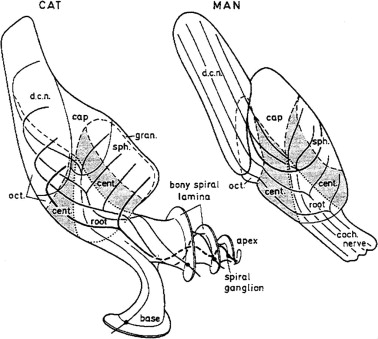
\includegraphics[width=2.25in,keepaspectratio]{gfx/Cat_Human_CN}}
    \caption{Cochlear nucleus innervation in Man and Cat. \citep[!find out which publication printed this!]{RyugoParks:2003,Ryugo:1992,Spoendlin:1973}}
    \label{fig:CNdiagram}
  \end{center}
\end{figure}


%\medskip{}

\todo[inline]{Discuss auditory model history. Expand reasons for wanting to create
  a biophysically realistic model of the CN\@. Discuss reason for using whole
  network in TV and TS optimisation}

%\medskip{}

\todo[inline]{a paragraph on the history of AN modelling
  \citep{LeakeSnyderEtAl:1993, ArnesenOsen:1978, CloptonWinfieldEtAl:1974}.
  Perhaps Rose et al 1959 would be better suited here}

%
%\medskip{}

In examining the properties of a detailed neural model of the cochlear nucleus,
a realistic and phenomenologically sound auditory model is needed to represent
sounds and transformations that occur in the central auditory system.

%
%\medskip{}
\subsection{Response of Carney auditory model }

The auditory nerve inputs to the cochlear nucleus model neurons are provided by
phenomenological auditory periphery models originating from
\citet{Carney:1993}. the ARLO model \citep{HeinzZhangEtAl:2001}; the Bruce model
\citep{BruceSachsEtAl:2003, ZilanyBruce:2006, ZilanyBruce:2007}; and the Zilany
model \citep{ZilanyBruceEtAl:2009}. The AN model consists of an outer/middle ear
pre-processing filter, a cochlea filterbank, IHC-to-AN synapse model and
dead-time modified Poisson spike generator, as shown in
Fig.~\ref{fig:ZilanyBruceFig}. \citep{HeinzZhangEtAl:2001} incorporated cochlea
filters based on the critical bandwidths obtained from psycho\-physical
experiments in humans. The ARLO model of the cat auditory periphery, with
non-linear compression and two-tone suppression, is used in this study except in
the vowel simulation where the human auditory periphery model is used.
\todo[inline]{TODO: AN model paragraph has been changed - fix any comment
  related to new Zilany}

%\medskip{}

% The \citet{ZilanyBruce:2007} model improves the previous AN model by an
% additional signal path and its predictions have matched a wide range of
% physiological data in normal and impaired cat data. The most recent AN model
% comprises an power-law synapse model, with internal $1/f$ noise, that enhances
% the behaviour of long-term dependence in ANFs \citep{ZilanyBruceEtAl:2009}.

%\medskip{}

% \todo[inline]{Why is it the cat model? updating Carney model?} Updating of the
% Carney auditory model has led to the change in the model's configuration from an
% original implementation of the rat model.  The default species is the cat and
% will be used in the data presented in this chapter.

 \begin{figure}[htb]
   \begin{center}
     \resizebox{3.5in}{!}{\includegraphics[keepaspectratio=true]{NoFigure}}
%     \resizebox{\textwidth}{!}{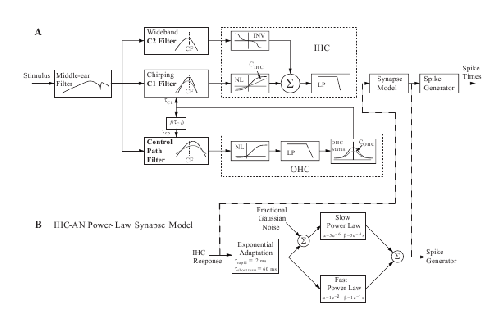
\includegraphics[keepaspectratio=true]{gfx/ZilanyCarney-JASA-2009-Fig2.eps}}
     \caption{Auditory periphery model with dual power-law synapse
       \citep[originally printed in ][]{ZilanyBruceEtAl:2009}.}
     \label{fig:ZilanyBruceFig}
   \end{center}
 \end{figure}\todo[inline]{if this figure is used it needs permission by the original authors}


\subsection{Spiking in Poisson neural models}

The neural models used in the auditory nerve fibres and Golgi cell model are
inhomogeneous Poisson processes. The instantaneous rate is passed through the
Jackson model, which includes refractory effects typical of the auditory nerve
fibres \citep{Jackson:2003,JacksonCarney:2005}.  Spike trains for each neuron in
the model are created at the start of each repetition of the stimulus, but can
be saved and loaded from file.




% \todo[inline]{TODO: serious reworking to be done here} 

%Analysis of the frequency
% response area of ANF generates known parameters for each fibre, these are:
% \begin{itemize}
% \item the spontaneous rate (SR), generated in silence and is
%   categoried into two groups High SR ($>$18 sp/s) and Low SR ($<$ 18
%   sp/s);
% \item threshold, the sound pressure level(SPL) at which the cell
%   responds above the spontaneous rate
% \item characteristic frequency (CF)
% \end{itemize}

%\medskip{}



% \begin{figure}[tbh]
%   \begin{center}
% %    \resizebox{3.5in}{!}{\includegraphics[keepaspectratio=true]{NoFigure}}
% %    \resizebox{3.5in}{!}{\includegraphics[keepaspectratio=true]{ClickDelay}}
%     \caption{Response of AN and CN cells to click stimuli. }
%     \label{fig:ClickDelayAN}
%   \end{center}
% \end{figure}


\section{Cochlear Nucleus Stellate microcircuit}

\subsection{Neural models}


\todo[inline]{[Discuss R\&M model] Is this a replication of other work or have I changed it enough that it needs to be shown or too general to go in this chapter (put in Methods Chapter}

%\medskip{}

\subsection{Tonotopic connectivity}\label{sec:tonot-conn}

The channels are separated using even spatial distance (based on the
basilar membrane and auditory nerve separation) with centre frequency
calculated by the Greenwood function for the cat
\citep{Greenwood:1990}. \todo[inline]{More detail in Appendix}

%\medskip{}

Figure~\ref{fig:CNconn} shows the method for Gaussian spread of
connections between cell types in the CN\@.  The channels are separated
using the same Greenwood function as used for the AN filterbank.


\begin{figure}[tbh]
  \begin{center}
%    \resizebox{3.5in}{!}{\includegraphics[keepaspectratio=true]{NoFigure}}
    \resizebox{\textwidth}{!}{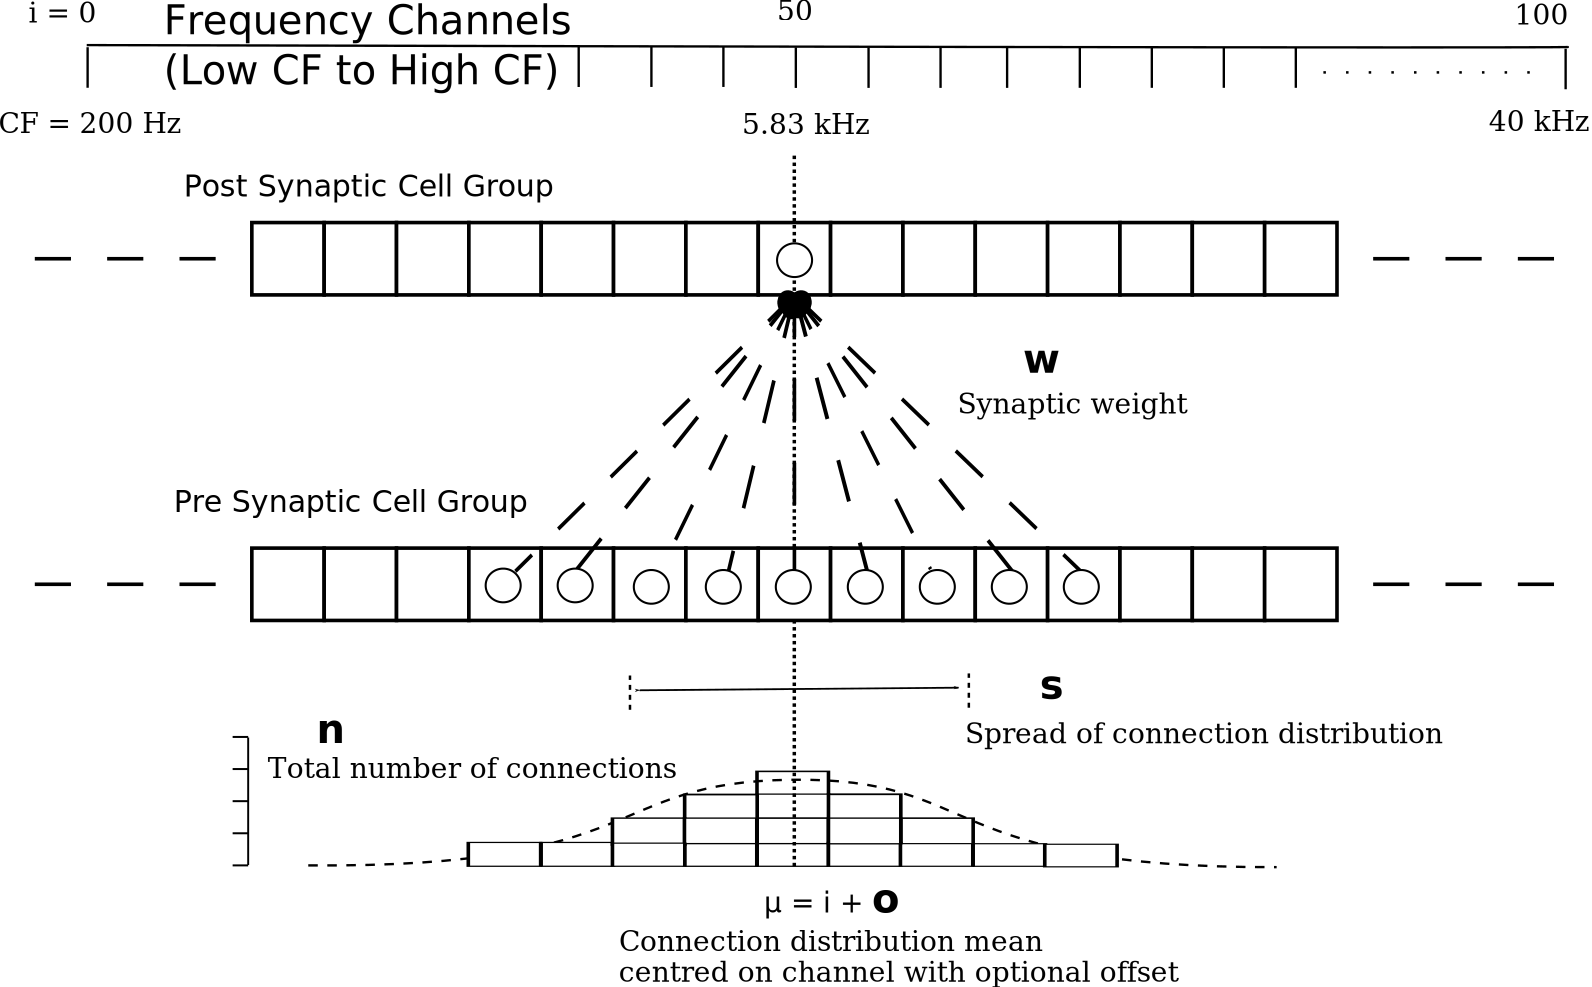
\includegraphics[keepaspectratio=true]{gfx/CNConn}}
%    \resizebox{0.8\textwidth}{!}{\input{./gfx/CNConn.tex}}
    \caption{Gaussian connection between cell types in cochlear
      nucleus.}
    \label{fig:CNconn}
  \end{center}
\end{figure}






%%% Local Variables: 
%%% mode: latex
%%% mode: tex-fold
%%% TeX-master: "SimpleResponses"
%%% TeX-PDF-mode: nil
%%% End: 

\newpage
{%
\small\linespread{0.5}
\noindent%
\begin{table}[!thb]
    \caption{Golgi cell model summary (Nordlie format)}
    \label{tab:GolgiCellModelSummary}
\begin{tabularx}{\textwidth}{|l|X|} %
\hdr{2}{A}{Model Summary}\\
%\begin{ntab}{|l|X|}{2}{\ref{tab:GolgiCellModelSummary} A}{Model Summary}\\\hline
 \textbf{Populations}  & ANF~(HSR, LSR) and Golgi (GLG) cells \\\hline 
  \textbf{Topology}    & Tonotopic - 100 frequency channels (0.2--40
  kHz);  Cat model; Greenwood function centre frequencies \citep{Greenwood:1990}\\\hline
\textbf{Connectivity}  & ANF to GLG filter inputs, Gaussian spread
centred on channel\\\hline
\textbf{Input model}  & ANF~model: Version 4 and 5 Zilany model \citep{ZilanyBruce:2007,ZilanyBruceEtAl:2009} \\\hline
\textbf{Neuron model}  & GLG cell model: Instantaneous-rate Poisson
neuron model \\\hline
\textbf{Synapse model} & Synapto-dendritic smoothing filter (alpha function) \\\hline
%    \textbf{Input}     & Pure tones (22.7 kHz, 50 ms, 5 ms on/off ramp, 20 ms delay), intensity range 0--100 dB~SPL   \\\hline
%\textbf{Measurements}  & Mean firing rate of Golgi cell instantaneous rate profile or PSTH sampled from Poisson spike-generator (25 repetitions) \\\hline
\end{tabularx}
\vspace{1ex}
%\end{ntab}

% - B ------------------------------------------------------------------------
\noindent%
\begin{tabularx}{\textwidth}{|l|X|X|}%
\hdr{3}{B}{Populations}\\
\textbf{Name} &                         \textbf{Elements}                          & \textbf{Number} \\\hline
     HSR      & Auditory nerve fibre model
     \citep{ZilanyBruce:2007,ZilanyBruceEtAl:2009} & Rate models only,
     1 per channel\\\hline
     LSR      & Auditory nerve fibre
     \citep{ZilanyBruce:2007,ZilanyBruceEtAl:2009} & Rate models only,
     1 per channel \\\hline
     GLG      &                 Instantaneous-rate Poisson neuron model                  & 1 unit (CF 22.7 kHz, channel 76)  \\\hline
\end{tabularx}
\vspace{1ex}

% - C ------------------------------------------------------------------------------
\noindent
\begin{tabularx}{\textwidth}{|l|l|l|X|}%
\hdr{4}{C}{Connectivity}    \\
     \textbf{Name}       & \textbf{Source} & \textbf{Target} & \textbf{Pattern} \\\hline
\multirow{2}{*}{\ANFGLG} &     {\HSR}      &      GLG      & 
Gaussian spatial convergence, centred on CF, spread parameter
(\sHSRGLG = 2). Weight (\wHSRGLG) to be optimised. \\
   &     {\LSR}      &      GLG      & 
Gaussian spatial convergence, centered on \CF.  Spread (\sLSRGLG) and weight (\wLSRGLG) to be optimised. \\\hline
\end{tabularx}
\vspace{1ex}
% - D ------------------------------------------------------------------------------
\noindent%
\begin{tabularx}{\linewidth}{|p{0.22\linewidth}|X|}
\hdr{2}{D}{Neuron and Synapse Model}\\
 \textbf{Name} & Golgi cell model \\\hline
 \textbf{Type} & Instantaneous-rate Poisson neural  model \\\hline 
%\raisebox{-4.5ex}{\parbox{\linewidth}{\textbf{Model Dynamics}}} & 
 \textbf{Model Dynamics} & %
% {\rule{1em}{0em}\vspace*{-1.5ex}\scriptsize%
% \begin{equation*}%
%  \begin{array}{r@{\;=\;}ll}
%   \mathbf{w}_{L,H}&  w_{LSR,HSR \to GLG}\,\mathcal{N}(i_{{\rm CF}},\sigma)    & \text{Gaussian weight mean at CF, \sigma^2=\sLSRGLG} \\ 
%   \alpha(t)      &\left( t  \exp(\frac{-t}{\Gtau}) \right)   &  \text{Synapto-dendritic filter with unit area} \\
%   g(t)           & \mathbf{w}_{L}\bullet\mathbf{L}+\mathbf{w}_{H}\bullet\mathbf{H} & \text{Sum of dot products} \\ % between weights and ANF rate matrices}\\ 
% %\mathbf{H},\mathbf{L} \to f(\text{channel},t) & \mathbf{w}_{H,L} \to f(\text{channel})\\
%              %      r(\mathbf{x})              &               \max\{\mathbf{x}(t-\dANFGLG) - x(0) + \Gspon,0\}                & \\
%  G(t)  &   \lfloor \, \alpha(t)\,\ast\,g(t) \,\rfloor                  & \text{Convolution of $\alpha(t)$ and $g(t)$ and rectification}\\
% % & \text{if } G(t) < 0 \,G(t)=0 & \text{rectification of Golgi model rate} \\
% \end{array} \end{equation*}\vspace*{-1.5ex}\rule{1em}{0em}}  \\\hline
%{\rule{1em}{0em}\vspace*{-1.5ex}%\scriptsize%
See Figure~\ref{fig:GolgiDiagram} and the GLG rate filter model
Equations~\ref{eq:GolgiWeights}--\ref{eq:GolgiConvolution}.
% ($g_{i}(t)$) used for
% the Golgi cell model. It was created using convolution of weighted ANF input rates
% and synapto-dendritic kernel ($\alpha_{\small\rm GLG}(t)$) with rectification. 
% \begin{equation*}%
%  \begin{array}{r@{\;=\;}l}
%  {\rm GLG}_{i}(t)  &  \alpha_{\rm GLG}(t)\,\ast\,g(t) \,\rfloor + \text{SR}_{\rm GLG} \quad \text{where} \\
%   \alpha(t)      &\left( t  \exp(\frac{-t}{\Gtau}) \right)   \quad  \text{and} \\
%   g(t)           & \mathbf{w}_{L}\bullet\mathbf{L}+\mathbf{w}_{H}\bullet\mathbf{H} 
% \end{array} \end{equation*}\vspace*{-1.5ex}\rule{1em}{0em}
%Preliminary rate, $g(t)$, is the sum of dot products between weight vectors and ANF rate matrices.
% Gaussian weight vectors have mean at CF and $\sigma^2=\sLSRGLG$.}  
\\\hline
 \textbf{Spiking} & Renewal Poisson process given instantaneous rate, ${\rm GLG}_{i}(t)$,  with refractory effects  \citep{ZilanyBruce:2007,Jackson:2003} \\\hline
\end{tabularx}
\vspace{2ex} 

% $\dag$\footnotesize{Synaptic filter, $\alpha(t)$, is normalised, by setting the
%   area under the alpha function to one. For a large enough filter length, the
%   alpha function integral ($\int \alpha(t) dt = (-\Gtau^2 - t \cdot \Gtau)\cdot
%   \exp(-\frac{t}{\Gtau})$) approximately equals $\Gtau^2$. In this case $10
%   \times \Gtau$ is used for the filter length.}  

% - E -----------------------------------------------------------------------------
\noindent
\begin{tabularx}{\linewidth}{|l|X|} %
\hdr{2}{E}{Optimisation}\\
\textbf{Input Stimulus} & Rate Level function, 22.7~kHz tone at SPL -15 to 90 dB (50 ms duration, 2 ms cosine squared on\slash off ramp, 20 ms delay)\\\hline 
\textbf{Parameters} & 
 \sANFGLG, 
   \Gtau,   
 \wHSRGLG,  
 \wLSRGLG,  
  \Gspon   \\\hline
\textbf{Fitness function}  & RMS squared error between rate-level functions of Golgi model (channel 76, CF=22.7 kHz) and unit S03-07 (CF=21 kHz) from \citet{GhoshalKim:1996}. Mean rate of Golgi model spikes sampled from 25 repetitions. \\\hline
\end{tabularx}
\vspace{1ex}
% \begin{ntab}{4}{|X|c|c|c|}{E}{Optimisation NTAB}
% \textbf{Parameters}             &    \textbf{Name}     & \textbf{Range} & \textbf{Best Values} \\\hline 
%  Spatial spread $\ANFGLG$ (channel unit)   &      $\sANFGLG$      &     [0,10]     & 2.48  \\\hline 
%  Synaptodendritic filter time constant (ms)     &   $\tau_{\ANFGLG}$     &     [0,20]       & 5.01  \\\hline 
%       Weighted sum of HSR (unitless)       &      $\wHSRGLG$      &     [0,5]      & 0.517 \\\hline 
%       Weighted sum of LSR (unitless)       &      $\wLSRGLG$      &     [0,5]      & 0.0487\\\hline 
% Golgi spontaneous rate (spikes per second) & \texttt{golgi\_spon} &     [0,50]     & 3.73  \\\hline
% \end{ntab}
\end{table}%
}

%%% Local Variables: 
%%% mode: latex
%%% TeX-master: "SimpleResponses"
%%% TeX-PDF-mode: nil
%%% End: 



%%%%%%%%%%%%%%%%%%%%%%%%%%%%%%%%%%%%%%%%%%%%%
\graphicspath{{/media/data/Work/cnstellate/golgi/}{/media/data/Work/Responses/}{/media/data/Work/cnstellate/Responses/}{../figures/}{./gfx/}}
%%%%%%%%%%%%%%%%%%%%%%%%%%%%%%%%%%%%%%%%%%%%%

\section[Golgi Cell Model]{Golgi Cell Model: Optimisation using
  monotonic rate-level responses in marginal shell units}
\label{sec:golgi-cell-model}
% Modelling in the auditory periphery has benefited extensively from
% the work of Liberman, Greewood, Patterson, Young, Sachs and others,
% in acoustic \texttt{in vivo} experiments.

\subsection{Background}

The source of GABAergic inputs to cells in the mammalian CN is
somewhat contentious. Despite studies showing that GABAergic inputs to
the CN generally arise in the peri-olivary regions of the medulla in
cats \citep{OstapoffBensonEtAl:1997} and birds
\citep{LachicaRubsamenEtAl:1995,YangMonsivaisEtAl:1999}, slice
preparations of the isolated murine VCN have shown sensitivity to
bicuculine in TS and DS cells \citep{FerragamoGoldingEtAl:1998a}.  The
only known source of GABA intrinsic to the VCN are the golgi cells of
the granule cell domain (GCD) overlying the VCN 
\citep[Fig.~\ref{fig:CNdiagram}]{Mugnaini:1985,FerragamoGoldingEtAl:1998}.
The presence of GABAergic inputs to TS, DS and TV cells has been
verified by labeled terminals adjacent to the soma and dendrites
\citep{SmithRhode:1989,AwatramaniTurecekEtAl:2005,BabalianRyugoEtAl:2003}
and release from inhibition in their response areas with
ionotopopheretic application of the \GABA antagonist, bicuculine
\citep{EvansZhao:1998,CasparyBackoffEtAl:1994,BackoffShadduckEtAl:1999,FerragamoGoldingEtAl:1998a}.

\medskip{}

Other studies in the rat cochlear nucleus relating to the Golgi cell or GABA:
\begin{itemize}
\item \citep{MugnainiOsenEtAl:1980} Fine structure of granule cells
  and related interneurons (termed {Golgi} cells) in the cochlear
  nuclear complex of cat, rat and mouse
\item GABAa expression in the rat brainstem  \citep{CamposCaboEtAl:2001}
\item \citep{Alibardi:2003a} Ultrastructural distribution of
  glycinergic and {{GABAergic}} neurons and axon terminals in the rat
  dorsal cochlear nucleus, with emphasis on granule cell areas
\item \citep{AwatramaniTurecekEtAl:2005} Staggered {Development} of
  {GABAergic} and {Glycinergic} {Transmission} in the {MNTB}
\end{itemize}

\medskip{}

Role of GABA in the VCN
\begin{itemize}
\item Effects of microiontophoretically applied glycine and {GABA} on
  neuronal response patterns in the cochlear nuclei
  \citep{CasparyHaveyEtAl:1979}
\end{itemize}

\citep{Alibardi:2003a} rat CN complex -> Golgi-stellate cells
(fusiform layer: 2) in DCN contact granule and unipolar brush cells


\medskip{}

Inputs to golgi cells are more complicated than VCN cells in the core
regions. Golgi cells are sparse in the GCD, surrounded by the many,
smaller excitatory granule cells, that form small en passant
endings. Type II ANFs create diffuse glutamatergic release sites in
the GCD \citep{HurdHutsonEtAl:1999,BensonBrown:2004} that may
stimulate NMDA glutamate receptors in golgi cells
\citep{FerragamoGoldingEtAl:1998a}.

\medskip{}

Extracellular recordings from the GCD by \citet{GhoshalKim:1997}, are most likely from golgi
cells since granule cell somata are less than  $10 \mu m$ and very
narrow axons. The majority of recorded
units showed a monotonic increase in firing rate with increasing sound
intensity \citep{GhoshalKim:1997}. 


\medskip{}

The lack of extensive experimental data meant that a phenomenological model
would be preferred over the Hogkin-Huxley type neural model. A number of steps
were taken to investigate the golgi cell model.

\medskip{}

The known GABAergic input to VCN units comes primarily from the superior olive
(ref), but the presence of active GABA synapses in isolated VCN slices by
\citet{FerragamoGoldingEtAl:1998} led to further investigation of
golgi cells in the granule cell domain. \citet{FerragamoGoldingEtAl:1998a}
showed that golgi cells have a classic type-I current
response, which suggest they integrate inputs, and their response to
AN shocks were delayed by approximately 0.7~ms relative to the core
VCN units .  Ghosal and Kim
\citet{GhoshalKim:1997} examined the VCN marginal shell in cats (equivalent to the
GCD in mice) that golgi cells provide some sort of
automatic gain control to the principle VCN units, through their monotonic
responses to tones and noise.

\medskip{}

% (Reference) showed that in adult animals high-spontaneous rate ANFs do not
% project to the GCD; they do show that low-spontaneous rate ANFs do project into
% the GCD, albeit more profusely than in the core on the VCN.
   

\begin{figure}[htb]
  \centering
\resizebox{0.8\textwidth}{!}{\includegraphics{NoFigure}}
%  \resizebox{0.8\textwidth}{!}{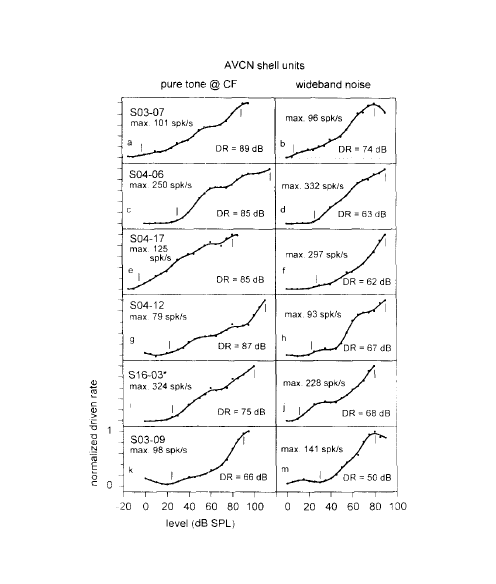
\includegraphics{GhoshalKim}}
\caption{Rate level response of unit S03-07 (CF 21~kHz) from Fig2
  \citep{GhoshalKim:1997} }
\end{figure}




\newpage
\subsection{Implementation}

In the creation of the golgi cell model, we can reduce the explicit
responses of Golgi cells down to three major details: a) golgi cells are integrators due to their type-I~current clamp response, b) golgi cells are (most likely) monotonic to tone and noise rate increases, and
c) they have a significant delay of first spike latency relative to the core VCN units.


In Chapter~\ref{sec:GAChapter} and previous publications \citep{EagerGraydenEtAl:2006a}, the golgi cell model was implemented as a single-compartment conductance  neuron. Due to the unavailability of sufficient data regarding \emph{in vivo}
golgi cell responses, we have decided to simulate the response of
golgi cells using inputs from the auditory model's instantaneous rate outputs rather
than simulating the neural membrane. 


The instantaneous rate vector of a golgi cell model at CF channel
\emph{i} is created by :
\begin{itemize}
 \item a selection of ANF input channels centred at \emph{i} with a
 spread, \sLSRGLG;
 \item the instantaneous rate vectors of the LSR ANF's in each channel
 are weighted (with a gaussian function (mean=\emph{i},
 s.d.=$\sqrt{\sLSRGLG}$) and the weighted vectors are averaged; and
 \item the weighted average vector is convolved with an alpha function
 of time constant 5, to simulate the synaptic and membrane dynamics of
 golgi cells
\end{itemize}

\medskip{}

\yellowbox{this needs to be removed}
[NEURON code methods] Each golgi cell template consists of a spike generator, \emph{s}, and vector
objects representing the instantaneous rate, the spike times and
accumulated  spike times of the golgi cell. Parameters identifying
each cell include the \emph{channel} number, CF and bandwidth of ANF
input (actually the variance of the weight each auditory filter
channel contributes to the firing of the cell).


\vspace{1ex}
% - A ------------------------------------------------------------------------



Monotonic rate-level data from GCD in VCN \citep{GhoshalKim:1996} unit
S03-07 (CF 21~kHz) was used to optimise parameters ${\rm
golgi\_spon}$, \wLSRGLG, \wHSRGLG, and \sANFGLG\@.  The optimisation
method was a default using the principle-axis method.
\medskip{}


Due to its replication of granule cells in the model, weight for LSR \wLSRGLG and HSR \wHSRGLG are determined for all synapses, number \nLSRDS and \nHSRDS, delay \dANFGLG added to smoothing function to ensure conductance and dendritic filtering are included.

\subsubsection{Key design factors}
 - Choosing neural model: HH-type or Poisson
 - Problem of monotonic excitation at low level
  - added HSR to model to avoid added computation of MSR
 - Spread of ANF to GCD ARE broader than core VCN
  - are we spoiling the broth too early? 


\begin{figure}[hp!]
  \centering
  \includegraphics[width=0.9\textwidth,trim=0 110mm 1 55mm]{gfx/GolgiDiagram}
  \caption{ The golgi instantaneous-rate profile was generated using ANF
    profiles. $\mu$ and $\sigma$ control the spread of connections
    across frequency channels, and $\mathbf{w}$ is
    the weighted sum of HSR and LSR instantaneous-rate vectors,
    $\alpha$ is the synaptic and dendritic smoothing function.}
\end{figure}


\noindent\begin{tabularx}{\linewidth}{|l|X|}\hline %
\hdr{2}{A}{Model Summary}\\\hline 
 \textbf{Populations}   & ANF(HSR,LSR) and Golgi \\\hline 
   \textbf{Topology}    & Tonotopic - 100 frequency channels based on Rat basilar membrane \citep{Greenwood:1990} and audiogram \citep{HeffnerHeffner:1985}\\\hline
 \textbf{Connectivity}  & Place-based Gaussian spread of connections \\\hline
 \textbf{Neuron model}  & ANFs: phenomenological instantaneous-rate Poisson model \citep{ZilanyBruceEtAl:2009} \\
& Golgi: instantaneous-rate Poisson model developed from ANF inputs\\\hline
\textbf{Channel models} & --- \\\hline 
\textbf{Synapse model}  & alpha function smoothing kernel \\\hline
\textbf{Input}      & Pure tones (21 kHz, 50 ms, 5 ms on/off ramp, 20 ms delay), 0-100 dB SPL  \\\hline
 \textbf{Measurements}  & Mean rate, spike activity \\\hline
\end{tabularx}

% - B ------------------------------------------------------------------------
\noindent\begin{tabularx}{\linewidth}{|l|X|X|}\hline %{\linewidth}
\hdr{3}{B}{Populations}\\\hline
  \textbf{Name}   & \textbf{Elements} & \textbf{Number} \\\hline
    HSR     & \citeauthor{ZilanyBruceEtAl:2009}  model        & $N_{\text{HSR}} = 50$ per freq.\ channel \\\hline
    LSR     & \citeauthor{ZilanyBruceEtAl:2009} model        & $N_{\text{LSR}}= 20$  per freq.\ channel \\\hline
    GLG     & Instantaneous rate Poisson model, spike-generator with refractory effects & $N_{\text{GLG}}= 1$  per freq.\ channel  \\\hline
\end{tabularx}
\vspace{1ex}

% - C ------------------------------------------------------------------------------
\noindent\begin{tabularx}{\linewidth}{|l|l|l|X|}\hline
\hdr{4}{C}{Connectivity}\\\hline
\textbf{Name} & \textbf{Source} & \textbf{Target} & \textbf{Pattern} \\\hline
  \multirow{2}{*}{$\textrm{ANF} \to \textrm{GLG}$} & LSR & Golgi &
  Gaussian spatial spread, centered at CF, variance determined by \sLSRGLG \\
 & HSR & Golgi & Fixed Gaussian spatial spread, centered at CF (\sHSRGLG =) \\\hline
 \end{tabularx}

\vspace{1ex}
% - D ------------------------------------------------------------------------------
\noindent\begin{tabularx}{\linewidth}{|l|X|}\hline
\hdr{2}{D}{Neuron and Synapse Model}\\\hline
            \textbf{Name}             & Golgi Phenomenological Model \\\hline
            \textbf{Type}             & Poisson instantaneous-rate model, ANF instantaneous rate input\\\hline
\multirow{4}{*}{\textbf{Golgi Model}} & $\mathbf{w}_{LSR} = N(\textrm{CF channel},\sLSRGLG)$,  $\mathbf{w}_{HSR} = N(\textrm{CF channel},\sHSRGLG)$  \\ 
                                      & $w(i,j) = \frac{1}{\sigma \sqrt{2\pi}} \exp \left\{-\frac{(i-j)^2}{2\sigma^2}\right\}, i,j \in [0,nchannels-1]$ \\
                                      & $\mathbf{g}_i = \sum^{i} w_{LSR}(i)\mathbf{L}_i + w_{HSR}(i)\mathbf{H}_i$ \\
                                      & $\mathbf{G}_i = \mathbf{g}_i * \alpha$  \\ \hline
\end{tabularx}
%\end{eqnarray}
% $\mathbf{w}_{LSR} = N(\textrm{CF channel},\sLSRGLG)$,  $\mathbf{w}_{HSR} = N(\textrm{CF channel},\sHSRGLG)$  \\ 
% &\texttt{for \textit{i}=0, nchannels} \\
% &	$\quad\mathbf{x}_i = \mathbf{w}_{LSR}(i)\cdot\mathbf{LSR}_i+\mathbf{w}_{HSR}(i)\cdot\mathbf{HSR}_i$ \\
% &\texttt{end} \\
% &	$\mathbf{x} = \mathbf{x}_i\circledast\mathbf{a}$  \texttt{//Convolve profile with Alpha kernel}\\\hline
% \multirow{3}{*}{\textbf{Spiking}} &
%    If $V(t-)<\theta \wedge V(t+)\geq \theta$
% \vspace*{-1ex}
% \begin{enumerate}\setlength{\itemsep}{-0.5ex}
% \item set $t^* = t$
% \item emit spike with time-stamp $t^*$
% \end{enumerate}
% \vspace*{-4ex}\rule{1em}{0em}
% \\\hline


% - E -----------------------------------------------------------------------------
\vspace{1ex}
\noindent\begin{tabularx}{\linewidth}{|l|X|}\hline %
\hdr{2}{E}{Input/Output}\\\hline 
\textbf{Input Stimulus} & Rate Level function, 21~kHz tone at SPL -15
to 85 dB (20 ms delay, 2ms cosine squared on/off ramp)\\\hline 
\textbf{Measurements}        & Mean rate of instantaneous rate profile or PSTH sampled from Poisson spike-generator (25 repetitions). \\\hline
\end{tabularx}
\vspace{1ex}



\noindent\begin{tabularx}{\linewidth}{|X|c|c|c|}\hline %{\textwidth}
\hdr{4}{F}{Optimisation} \\ \hline 
     \textbf{Parameters}      &  \textbf{Name}   & \textbf{Range} & \textbf{Best Values} \\\hline 
   Spatial spread $\ANFGLG$ (channel units)    &     $\sANFGLG$     &     [0,10]     & 2.48 \\\hline 
Dendritic Filter time constant (ms)& $\tau_{\ANFGLG}$ &    [0,20]   & 5.01\\\hline 
     Weighted sum of HSR (unitless)     &    $\wHSRGLG$    &      [0,5]     & 0.517 \\\hline 
     Weighted sum of HSR (unitless)     &    $\wLSRGLG$    &      [0,5]     & 0.0487\\\hline 
     Golgi spontaneous rate (spikes per second)       &  \texttt{golgi\_spon} &  [0,50]  & 3.73 \\\hline
\end{tabularx}




% \includegraphics[width=0.6\textwidth,angle=-90]{GolgiRateLevelActualFit}\\
% \caption{Optimisation Results for Golgi Model using Rate Level data
%   from }\label{Ch3:fig:GolgiFit}
% \includegraphics[width=0.8\textwidth]{GolgiRateLevel}\\
% \caption{Optimisation Results for Golgi Model using Rate Level data
%   from }\label{Ch3:fig:GolgiRL}

% \includegraphics[width=0.8\textwidth]{golgi_RateLevel_opt}\\
% \caption{Optimisation Results for Golgi Model using Rate Level data
%   from }\label{Ch3:fig:GolgiRL}
% \includegraphics[width=0.8\textwidth,angle\todo=-90]{GolgiRateLevel2}\\
% \caption{Optimisation Results for Golgi Model using Rate Level data
%   from }\label{Ch3:fig:GolgiRL}

\clearpage
\subsection{Results}
Fig. 4: Golgi model (Green) and spike based output (Pink) was used to
fit the experimental data of unit S03-07 (CF 21~kHz) from
\citep{GhoshalKim:1996} (Red).  LSR mean rate (Blue) of 21~kHz unit is
monotonic with a high threshold.



\begin{figure}[htb]
  \centering \turnbox{90}{\small{Rate (sp/s)}}
%  \resizebox{0.8\textwidth}{!}{\includegraphics[angle=-90]{GolgiRateLevel2}}\\
  \caption{Rate Level (dB SPL)}
\end{figure}


\textbf{Error} 0.021 (MSE re max rate)



%   % \includegraphics[width=0.6\textwidth,angle=-90]{GolgiRateLevelActualFit}\\
%   % \caption{Optimisation Results for Golgi Model using  Rate Level data from }\label{Ch3:fig:GolgiFit}
%   % \includegraphics[width=0.8\textwidth]{GolgiRateLevel}\\
%   % \caption{Optimisation Results for Golgi Model using  Rate Level data from }\label{Ch3:fig:GolgiRL}

%   % \includegraphics[width=0.8\textwidth]{golgi_RateLevel_opt}\\
%   % \caption{Optimisation Results for Golgi Model using  Rate Level data from }\label{Ch3:fig:GolgiRL}
%   % \includegraphics[width=0.8\textwidth,angle=-90]{GolgiRateLevel2}\\
%     % \caption{Optimisation Results for Golgi Model using  Rate Level data from }\label{Ch3:fig:GolgiRL}





% \begin{figure}[htb]
% \centering
%   \includegraphics[width=0.6\textwidth,angle=-90]{GolgiRateLevelActualFit}\\
%   \caption{Optimisation Results for Golgi Model using  Rate Level data from }\label{Ch3:fig:GolgiFit}
% \end{figure}

% \begin{figure}[htb]
% \centering
%   \includegraphics[width=0.8\textwidth]{GolgiRateLevel}\\
%   \caption{Optimisation Results for Golgi Model using  Rate Level data from }\label{Ch3:fig:GolgiRL}
% \end{figure}

% \begin{figure}[htb]
% \centering
%   \includegraphics[width=0.8\textwidth]{golgi_RateLevel_opt}\\
%   \caption{Optimisation Results for Golgi Model using  Rate Level data from }\label{Ch3:fig:GolgiRL}
% \end{figure}

% \begin{figure}[htb]
% \centering
%   \includegraphics[width=0.8\textwidth,angle=-90]{GolgiRateLevel2}\\
%   \caption{Optimisation Results for Golgi Model using  Rate Level data from }\label{Ch3:fig:GolgiRL}
% \end{figure}





% \clearpage \newpage
\section{Verification}

 \subsection{Tone Response}

% \begin{figure}[h]
%   \centering\resizebox{0.95\textwidth}{!}{%
%     \includegraphics{RateLevel/psthsingle90.3.eps}%
%     \includegraphics{RateLevel/G_ratelevel.eps}}
% \end{figure}
% \begin{figure}[h]
%   \centering\resizebox{0.95\textwidth}{!}{%
%     \includegraphics{RateLevel/response_area.3.eps}%
%     \includegraphics{RateLevel/response_area_log2.3.eps}}
% \end{figure}
% \begin{figure}[h]
%   \centering\resizebox{0.95\textwidth}{!}{%
%     % \includegraphics{RateLevel/response_area.3.eps}
%     \includegraphics{RateLevel/psthall90.3.eps}%
%     \includegraphics{RateLevel/psthVlevel.3.eps}}
% \end{figure}



% \clearpage
 \subsection{Noise Response}
% \begin{figure}[h]
%   \centering\resizebox{0.95\textwidth}{!}{%
%     \includegraphics{NoiseRateLevel/psthsingle120.3.eps}%
%     \includegraphics{NoiseRateLevel/G_ratelevel.eps}}
% \end{figure}
% \begin{figure}[h]
%   \centering\resizebox{0.95\textwidth}{!}{%
%     \includegraphics{NoiseRateLevel/response_area.3.eps}%
%     \includegraphics{NoiseRateLevel/response_area_log2.3.eps}}
% \end{figure}
% \begin{figure}[h]
%   \centering\resizebox{0.95\textwidth}{!}{%
%     % \includegraphics{RateLevel/response_area.3.eps}
%     \includegraphics{NoiseRateLevel/psthall90.3.eps}%
%     \includegraphics{NoiseRateLevel/psthVlevel.3.eps}}
% \end{figure}


% \clearpage
 \subsection{Masked Noise and Tone}
% \begin{figure}[h!]
%   \centering\resizebox{0.95\textwidth}{!}{\includegraphics{MaskedRateLevel/psthsingle90.3.eps}\includegraphics{MaskedRateLevel/G_ratelevel.eps}}
% \end{figure}
% \begin{figure}[h!]
%   \centering\resizebox{0.95\textwidth}{!}{%
%     \includegraphics{MaskedRateLevel/response_area.3.eps}%
%     \includegraphics{MaskedRateLevel/response_area_log2.3.eps}}
% \end{figure}

% \begin{figure}[h!]
%   \centering\resizebox{0.95\textwidth}{!}{%
%     % \includegraphics{RateLevel/response_area.3.eps}
%     \includegraphics{MaskedRateLevel/psthall90.3.eps}%
%     \includegraphics{MaskedRateLevel/psthVlevel.3.eps}}
% \end{figure}
% \clearpage
 \subsection{Masked Response Area}
% \begin{figure}[h!]
%   \centering\resizebox{0.95\textwidth}{!}{%
%     \includegraphics{MaskedResponseCurve/psthsingle5810.3.eps}%
%     \includegraphics{MaskedResponseCurve/G_masked.eps}}
% \end{figure}
% \begin{figure}[h!]
%   \centering\resizebox{0.95\textwidth}{!}{%
%     \includegraphics{MaskedResponseCurve/response_area.3.eps}%
%     \includegraphics{MaskedResponseCurve/response_area_log2log2.3.eps}}
% \end{figure}

% \begin{figure}[h!]
%   \centering\resizebox{0.95\textwidth}{!}{%
%     % \includegraphics{RateLevel/response_area.3.eps}
%     \includegraphics{MaskedResponseCurve/psthall5810.3.eps}%
%     \includegraphics{MaskedResponseCurve/psthVmod.3.eps}}
% \end{figure}
% \clearpage


% \todo{add stuff here}



% % %%%%%%%%%%%%%%%%%%%%%%%%%%%%%%%%%%%%%%%%%%%%%%%%%%%%%%
% \bibliographystyle{plainnat}%bmc_article} % Style BST file
% \bibliography{../manuscript/bib/MyBib}
 
% \end{document}





%%% Local Variables: 
%%% mode: latex
%%% TeX-master: "SimpleResponses"
%%% TeX-PDF-mode: nil
%%% End: 

\newpage
{\small%\linespread{0.5}
  \begin{table}[ht]
    \caption{D~stellate cell  model summary}
    \label{tab:DScellModelSummary}
  \end{table}
\noindent%
\begin{tabularx}{\textwidth}{|l|X|}\hline %
\hdr{2}{A}{Model Summary}\\\hline
         \textbf{Populations}          & ANF (HSR,LSR), Golgi, and  D~stellate cells\\\hline
          \textbf{Topology}            & Tonotopic, auditory system of the rat  \\\hline
        \textbf{Connectivity}          & Gaussian spread dependent on morphology and afferent connections  \\\hline
         \textbf{Input model}          & Auditory nerve model \citep{ZilanyBruce:2007}\\\hline
\multirow{2}{*}{\textbf{Neuron model}} & Golgi: instantaneous-rate Poisson spike trains\\
                                       & D~stellate: Type 1-2 R\&M single compartment neuron\\ \hline
       \textbf{Channel models}         & $I_{\textrm{Na}}$, $I_{\textrm{KHT}}$, $I_{\textrm{KLT}}$, $I_{\textrm{KA}}$ and $I_{\textrm{h}}$ \citep{RothmanManis:2003b} \\\hline
        \textbf{Synapse model}         & Conductance synapses: excitatory (single-exponential), GABAergic (double-exponential) \\\hline
       \textbf{Input Stimulus}         & Mask/Recovery click trains with delay 2, 3, 4 and 8
ms, separated by 50 ms\\\hline
        \textbf{Measurements}          & PSTH sampled at each recovery click for 2 ms to measure click recovery\\\hline
% PSTHs were generated from 25
%   stimulus repetitions. Each response to a click is measured for 2 ms
%   after the minimum first spike latency for the unit.  The unit used
%   in the optimisation has a CF = 5.8~kHz (channel no. 50).\\ \hline
\end{tabularx}
\vspace{2ex}

% - B -----------------------------------------------------------------------------

\noindent%
\begin{tabularx}{\textwidth}{|l|X|X|}\hline %{\textwidth}
\hdr{3}{B}{Populations}\\\hline
\textbf{Name} &               \textbf{Elements}                & \textbf{Number} \\\hline
     HSR      & Auditory nerve fibre \citep{ZilanyBruce:2007}  & $N_{\text{HSR}} = 50\times{}N_\mathsf{channel}$ \\\hline
     LSR      & Auditory nerve fibre \citep{ZilanyBruce:2007}  & $N_{\text{LSR}} = 20\times{}N_\mathsf{channel}$ \\\hline
     GLG      & Instantaneous-rate Poisson neuron        & $N_{\text{GLG}} = 1\times{}N_\mathsf{channel}$ \\\hline
     DS       & Type I-II \citeauthor{RothmanManis:2003b} model & 1 unit at channel 50, $CF = 5.6$ kHz \\\hline
\end{tabularx}
\vspace{2ex}

% - C ------------------------------------------------------------------------------

\noindent%
\begin{tabularx}{\textwidth}{|l|l|l|X|}\hline
\hdr{4}{C}{Connectivity}\\\hline
        \textbf{Name}          & \textbf{Source} & \textbf{Target} & \textbf{Pattern} \\\hline
$\textrm{HSR} \to \textrm{DS}$ &       ANF       &   D~Stellate    & skewed Gaussian, centered at CF, spread below CF \sANFDSl, spread above CF \sANFDSh, uniform weight \wANFDS\ for all synapses, number \nLSRDS\ and \nHSRDS, delay \dANFDS \\\hline
$\textrm{LSR} \to \textrm{DS}$ &       ANF       &   D~Stellate    & skewed Gaussian, centered at CF, spread below CF \sANFDSl, spread above CF \sANFDSh, uniform weight \wANFDS\ for all synapses, number \nLSRDS\ and \nHSRDS, delay \dANFDS \\\hline

$\textrm{GLG} \to \textrm{DS}$ &      Golgi      &   D~Stellate    & Gaussian, centered at CF with spread \sGLGDS, uniform weight \wGLGDS, number \nGLGDS, delay \dGLGDS \\\hline
\end{tabularx}

\vspace{2ex}




% - D ------------------------------------------------------------------------------

\noindent%
\begin{tabularx}{\textwidth}{|l|X|}\hline
\hdr{2}{D}{Neuron and Synapse Model}\\\hline
 \textbf{Name} & DS cell model \\\hline
 \textbf{Type} & Type 1-2 \citep{RothmanManis:2003b}, conductance synapse input \\\hline
 \textbf{Spiking} & Emit spike when $V(t)\geq \theta$  \\\hline
 \end{tabularx}

\vspace{2ex}
}


%%% Local Variables: 
%%% mode: latex
%%% TeX-master: "SimpleResponses"
%%% TeX-PDF-mode: nil
%%% End: 


\graphicspath{{/media/data/Work/cnstellate/DS_ClickRecovery/}{/media/data/Work/Responses/}{../figures/}{./gfx/}}
\section[DS Cell Model]{D-Stellate Cell Model: optimisation using click recovery responses}
\label{sec:d-stellate-cell-model}

\subsection{Introduction}

This section shows the GABAergic input and intrinsic cell properties
influence the behaviour Onset chopper units.  Onset-chopper units in
the mammalian VCN have a wide-ranging influence on the primary cells
of the VCN (stellate and bushy neurons \citep{RhodeSmithEtAl:1983}),
the ipsilateral DCN (type II and type IV EIRA units) and the
contra\-lateral CN \citep{NeedhamPaolini:2007}.

\medskip{}


% Large multipolar or stellate cells in the VCN have been shown to have
% 3-4 long dendrites stretching 200 microns (or one third of the VCN)
% and their axonal collaterals cover the same region in the VCN, almost
% one half of the DCN, and are one source of the commisural projection
% to the contralateral cochlear nucleus \citep{NeedhamPaolini:2007}.
%%%%%%%%%%%%%%%%%%%Copied from original jneurometh article
  
D-stellate (DS) cells are large multipolar neurons in the VCN and have an
onset-chopping (On-C) PSTH to tones and noise \citep{SmithRhode:1989,
  NeedhamPaolini:2006}.  They typically have 3-4 long dendrites stretching 200
microns (or one third of the VCN) and their axonal collaterals cover the same
region in the VCN, almost one half of the DCN, and are one source of the
commisural projection to the contralateral cochlear nucleus
\citep{Cant:1992,Cant:1981,SchofieldCant:1996,CantBenson:2003,
  NeedhamPaolini:2007, PaoliniClark:1999}. Intracellular responses to sounds
indicate the bandwidth of inputs to DS neurons typically ranges from two octaves
below CF to one octave above CF \citep{PalmerJiangEtAl:1996,
  JiangPalmerEtAl:1996, PaoliniClark:1999}. DS cell axon terminals contain the
inhibitory neurotransmitter glycine and synapse widely in the VCN and DCN\@.
They also send a commissural projection to the contralateral cochlear nucleus
that mediates fast inhibition between the nuclei \citep{NeedhamPaolini:2003,
  NeedhamPaolini:2006, Oertel:1997}.


\medskip{}

Post-onset GABAergic inhibition in DS cells is a major influence on the PSTH of
On-C neurons \citep{FerragamoGoldingEtAl:1998a,EvansZhao:1998}. Latency of
excitation to auditory nerve shocks suggests golgi cells are activated by type
II ANFs and low spontaneous rate type I ANFs \citep{BensonBerglundEtAl:1996,
  FerragamoGoldingEtAl:1998}. Therefore, type II and LS type I ANFs could be
involved in gain control through GABAergic modulation of activity in the VCN.

\medskip{}

\yellownote{Discuss AM coding by DS cells} GABA blockers in the VCN has the
effects of changing the behaviour in the response to AM in the IC
\citep{CasparyPalombiEtAl:2002}.  AM coding effects of GABA in the Chinchilla CN
\citep{BackoffShadduckEtAl:1999}.  \citep{CasparyBackoffEtAl:1994} Caspary and
colleagues worked on the effects of GABA in in the VCN\@.

Zhang and Winter looked at the response area of VCN onset units to
determine GABA on/off freq. 

Smith and Rhode, Smith and others looked at OnC response area and two-tone



\subsection{Implementation}
 
Key factors in designing D-stellate cell model

\medskip{}

Choosing neural model: type I-II Rothman and Manis model
  - with/without dendrites: dendrites are 
  - variable KLT, leak conductance

\begin{itemize}
\item  ANF spread to DS cells well documented (decision made to
    fix params due to large computational task of calc response area) 
\item  short delay recovery responses (2,3,4 ms) were not successful upon
    first model, included DS leak and KLT conductances to allow cell
    behaviour to be fit
\item The effect of Golgi cells on DS is delayed by the extra 0.7 ms
    delay from ANF to Golgi, plus the slow peak of \GABAa inhibition.
\end{itemize}

\medskip{}

Optimisation parameters for \GLGDS are optimised based on experimental
click recovery data from \citep{BackoffPalombiEtAl:1997}.  Fixed
parameters included the number of golgi cells to DS cells ($\nGLGDS =
25$), the spread of ANFs to DS cells $\ANFDS$, and the extra delay
from the auditory nerve.  The first spike latency in DS cells 2.8 ±
0.09 ms \citep{RhodeSmith:1986}.The addition of 0.5 ms to \ANFDS
connections is a combination of conductance and synaptic delay. The
effect of Golgi cells on DS is delayed by the extra 0.7~ms delay from
ANF to Golgi, plus the slow peak of \GABAa inhibition.  The spread ANF
to DS cells (\sANFDSh,\sANFDSl) is arbitrary at this point and fairly
broad so the estimate is set so that 2 octaves below and 1 octave
above CF are within 2 standard deviations \citep{PaoliniClark:1999}.
\medskip{}

The optimisation function was a weighted mean squared error between
the experimental and simulated data, from an array where the elements
were the number of spikes in a 2 ms window after a click.  The input
stimulus was a series of masker/response clicks, with the click
intervals of 2, 3, 4, 8, 16 ms, and a separation of 50 ms.


 PSTHs were generated from 25
   stimulus repetitions. Each response to a click is measured for 2 ms
   after the minimum first spike latency for the unit.  The unit  used
   in the optimisation has a CF of 5.8~kHz (equivalent to channel no. 50).


% \begin{figure}[htb]
%   \centering
% \includegraphics[width=0.5\textwidth]{DS_ClickRecovery_DSpsth}\label{fig:DSClickRecoveryPSTH}\\
% \includegraphics[width=0.5\textwidth]{DS_ClickRecovery_Gpsth}\label{fig:GClickRecoveryPSTH}
%    \caption{PSTH response of a D-stellate cell from the click recovery stimulus used in the optimisation.}
%  \end{figure}



 % ---------------------------------------------------------------------------------
 \newpage
% \begin{lstlisting}
% func fun() {local f
%       //Modify Variables
%       param.w.x[glg][ds] = $2
%       param.w.x[hsr][ds] = $3
%       param.w.x[lsr][ds] = $3
%       //Modify the network
%       {create_cells() connect_cells(fileroot) SetRates()}
%       // Simulate the network for N reps
%       for j=0, reps-1{
%          print j
%          GenSpikes()
%          run()
%          DSvec.append(dstellate[50][0].spiketimes)
%          //print startsw()-x, "secs"
%       }
%       DSvec = DSvec.histogram(0,tstop,0.1)
%
%       objref errorvec
%       errorvec = new Vector()
%       //Find the mean number of spikes in the first click
%       maxrate = (DSvec.sum(240,260) + DSvec.sum(740,760)+ DSvec.sum(1340,1360))/3
%       //Calc ratio of number of spikes in second click relative to mean first click
%       errorvec.append( DSvec.sum(260,280) / maxrate )
%       errorvec.append( DSvec.sum(780,800) / maxrate )
%       errorvec.append( DSvec.sum(1420,1440) / maxrate )
%       errorvec.plot(g
%     return errorvec.meansqerr(targetclick)
% }
% \end{lstlisting}


{\small%\linespread{0.5}
  \begin{table}[ht]
    \caption{D~stellate cell  model summary}
    \label{tab:DScellModelSummary}
  \end{table}
\noindent%
\begin{tabularx}{\textwidth}{|l|X|}\hline %
\hdr{2}{A}{Model Summary}\\\hline
         \textbf{Populations}          & ANF (HSR,LSR), Golgi, and  D~stellate cells\\\hline
          \textbf{Topology}            & Tonotopic, auditory system of the rat  \\\hline
        \textbf{Connectivity}          & Gaussian spread dependent on morphology and afferent connections  \\\hline
         \textbf{Input model}          & Auditory nerve model \citep{ZilanyBruce:2007}\\\hline
\multirow{2}{*}{\textbf{Neuron model}} & Golgi: instantaneous-rate Poisson spike trains\\
                                       & D~stellate: Type 1-2 R\&M single compartment neuron\\ \hline
       \textbf{Channel models}         & $I_{\textrm{Na}}$, $I_{\textrm{KHT}}$, $I_{\textrm{KLT}}$, $I_{\textrm{KA}}$ and $I_{\textrm{h}}$ \citep{RothmanManis:2003b} \\\hline
        \textbf{Synapse model}         & Conductance synapses: excitatory (single-exponential), GABAergic (double-exponential) \\\hline
       \textbf{Input Stimulus}         & Mask/Recovery click trains with delay 2, 3, 4 and 8
ms, separated by 50 ms\\\hline
        \textbf{Measurements}          & PSTH sampled at each recovery click for 2 ms to measure click recovery\\\hline
% PSTHs were generated from 25
%   stimulus repetitions. Each response to a click is measured for 2 ms
%   after the minimum first spike latency for the unit.  The unit used
%   in the optimisation has a CF = 5.8~kHz (channel no. 50).\\ \hline
\end{tabularx}
\vspace{2ex}

% - B -----------------------------------------------------------------------------

\noindent%
\begin{tabularx}{\textwidth}{|l|X|X|}\hline %{\textwidth}
\hdr{3}{B}{Populations}\\\hline
\textbf{Name} &               \textbf{Elements}                & \textbf{Number} \\\hline
     HSR      & Auditory nerve fibre \citep{ZilanyBruce:2007}  & $N_{\text{HSR}} = 50\times{}N_\mathsf{channel}$ \\\hline
     LSR      & Auditory nerve fibre \citep{ZilanyBruce:2007}  & $N_{\text{LSR}} = 20\times{}N_\mathsf{channel}$ \\\hline
     GLG      & Instantaneous-rate Poisson neuron        & $N_{\text{GLG}} = 1\times{}N_\mathsf{channel}$ \\\hline
     DS       & Type I-II \citeauthor{RothmanManis:2003b} model & 1 unit at channel 50, $CF = 5.6$ kHz \\\hline
\end{tabularx}
\vspace{2ex}

% - C ------------------------------------------------------------------------------

\noindent%
\begin{tabularx}{\textwidth}{|l|l|l|X|}\hline
\hdr{4}{C}{Connectivity}\\\hline
        \textbf{Name}          & \textbf{Source} & \textbf{Target} & \textbf{Pattern} \\\hline
$\textrm{HSR} \to \textrm{DS}$ &       ANF       &   D~Stellate    & skewed Gaussian, centered at CF, spread below CF \sANFDSl, spread above CF \sANFDSh, uniform weight \wANFDS\ for all synapses, number \nLSRDS\ and \nHSRDS, delay \dANFDS \\\hline
$\textrm{LSR} \to \textrm{DS}$ &       ANF       &   D~Stellate    & skewed Gaussian, centered at CF, spread below CF \sANFDSl, spread above CF \sANFDSh, uniform weight \wANFDS\ for all synapses, number \nLSRDS\ and \nHSRDS, delay \dANFDS \\\hline

$\textrm{GLG} \to \textrm{DS}$ &      Golgi      &   D~Stellate    & Gaussian, centered at CF with spread \sGLGDS, uniform weight \wGLGDS, number \nGLGDS, delay \dGLGDS \\\hline
\end{tabularx}

\vspace{2ex}




% - D ------------------------------------------------------------------------------

\noindent%
\begin{tabularx}{\textwidth}{|l|X|}\hline
\hdr{2}{D}{Neuron and Synapse Model}\\\hline
 \textbf{Name} & DS cell model \\\hline
 \textbf{Type} & Type 1-2 \citep{RothmanManis:2003b}, conductance synapse input \\\hline
 \textbf{Spiking} & Emit spike when $V(t)\geq \theta$  \\\hline
 \end{tabularx}

\vspace{2ex}
}


%%% Local Variables: 
%%% mode: latex
%%% TeX-master: "SimpleResponses"
%%% TeX-PDF-mode: nil
%%% End: 



\clearpage

\begin{figure}[htb]
\centering
\resizebox{5in}{!}{\includegraphics{NoFigure}}
%\includegraphics[keepaspectratio,angle=-90,width=0.8\textwidth]{DSClickRecoveryExpData}
\caption{Experimental Data of GABAergic influence on D-stellate cells from \citep{BackoffPalombiEtAl:1997}, Fig.~3.}\label{Ch3:fig:DSClickRecoveryExpData}
\end{figure}

%\parsep

\clearpage
\subsection{Results}

% \noindent\begin{tabularx}{\textwidth}{|l|X|}\hline %{\textwidth}
% \hdr{2}{D}{Results} \\\hline
% \end{minipage}}\\\hline
% \textbf{Error} & 0.006671    unweighted (MSE of recovery spike rate / mask rate)\\\hline
% & 0.01447    final result (MSE of recovery spike rate / mask rate)\\\hline
% \end{tabularx}

\begin{figure}[htb!]
  \centering
\resizebox{0.9\textwidth}{!}{\includegraphics{NoFigure}}
%\resizebox{3.5in}{!}{\includegraphics[angle=-90]{./gfx/DS_ClickRecovery_result.eps}}
\caption{Experimental Data ({\color{green} Green}) of GABAergic influence on D-stellate cells from \citep{BackoffPalombiEtAl:1997}, Fig.~3.  Best result ({\color{blue} Blue}) shown in figure below.} \label{fig:DS_ClickRecovery_result}  
\end{figure}


% \begin{figure}
%   \includegraphics[width=0.5\textwidth]{DS_ClickRecovery_OptVars.eps}\\
% %  \includegraphics[width=0.5\textwidth]{DS_ClickRecovery_Output.eps}\label{Ch3:fig:DSClickRecoveryOutput}
%   \caption{Final Output Data of the D-stellate Click Recovery optimisation }
% \end{figure}

% \begin{figure}
%   \includegraphics[keepaspectratio=true,width=0.8\textwidth]{DS_ClickRecovery_Example1.eps}\\
%   \includegraphics[keepaspectratio=true,width=0.8\textwidth]{DS_ClickRecovery_Example10.eps}\\
%   \includegraphics[keepaspectratio=true,width=0.8\textwidth]{DS_ClickRecovery_Example13.eps}\\
%   \includegraphics[keepaspectratio=true,width=0.8\textwidth]{DS_ClickRecovery_Example19.eps}\\
%   \caption{Click Recovery optimisation functions}
% \end{figure}




% \begin{figure}
%   \includegraphics[keepaspectratio=true,angle=-90,width=0.8\textwidth]{DS_ClickRecovery_result1.eps}\\
% \end{figure}


% \begin{figure}
%   \includegraphics[keepaspectratio=true,angle=-90,width=0.8\textwidth]{DS_ClickRecovery_result2.eps}\\
%   \caption{Click Recovery optimisation }
% \end{figure}




% \begin{figure}
% \begin{center}
% \includegraphics[keepaspectratio=true]{DS_ClickRecovery_handtuned.eps}\\
% \includegraphics[keepaspectratio=true,angle=-90,width=0.8\textwidth]{DS_ClickRecovery_result_handtuned.eps}
% \caption{Handtuned}
% \label{hantuned}
% \end{center}
% \end{figure}

% \begin{figure}
% \begin{center}
% %\includegraphics[keepaspectratio=true]{DS_ClickRecovery_handtuned.eps}\\
% \includegraphics[keepaspectratio=true,angle=-90,width=0.8\textwidth]{gfx/DS_ClickRecovery_result_unweighted_8.eps}\\
% \includegraphics[keepaspectratio=true,angle=-90,width=0.8\textwidth]{gfx/DS_ClickRecovery_result_weighted_0.eps}
% \caption{Handtuned}
% \label{hantuned}
% \end{center}
% \end{figure}

 \clearpage
%\newpage
\subsection{Verification}

 \subsection{Tone Responses}
% \begin{figure}[h!]
% \centering\resizebox{\textwidth}{!}{%
% \includegraphics{RateLevel/psthsingle90.2.eps}%
% \includegraphics{RateLevel/DS_ratelevel.eps}}
% \end{figure}
% \begin{figure}[h!]
% \centering\resizebox{\textwidth}{!}{%
% \includegraphics{RateLevel/response_area.2.eps}%
% \includegraphics{RateLevel/response_area_log2.2.eps}}
% \end{figure}
% \begin{figure}[h!]
% \centering\resizebox{\textwidth}{!}{%
% %\includegraphics{RateLevel/response_area.2.eps}
% \includegraphics{RateLevel/psthall90.2.eps}%
% \includegraphics{RateLevel/psthVlevel.2.eps}}
% \end{figure}


% \clearpage
 \subsection{Noise Responses}
% \begin{figure}[h!]
% \centering\resizebox{\textwidth}{!}{%
% \includegraphics{NoiseRateLevel/psthsingle120.2.eps}%
% \includegraphics{NoiseRateLevel/DS_ratelevel.eps}}
% \end{figure}
% \begin{figure}[h!]
% \centering\resizebox{\textwidth}{!}{%
% \includegraphics{NoiseRateLevel/response_area.2.eps}%
% \includegraphics{NoiseRateLevel/response_area_log2.2.eps}}
% \end{figure}
% \begin{figure}[h!]
% \centering\resizebox{\textwidth}{!}{%
% %\includegraphics{RateLevel/response_area.2.eps}
% \includegraphics{NoiseRateLevel/psthall90.2.eps}%
% \includegraphics{NoiseRateLevel/psthVlevel.2.eps}}
% \end{figure}


% \clearpage
 \subsection{Masked Noise and Tone Responses}
% \begin{figure}[h!]
% \centering\resizebox{\textwidth}{!}{\includegraphics{MaskedRateLevel/psthsingle90.2.eps}\includegraphics{MaskedRateLevel/DS_ratelevel.eps}}
% \end{figure}
% \begin{figure}[h!]
% \centering\resizebox{\textwidth}{!}{%
% \includegraphics{MaskedRateLevel/response_area.2.eps}%
% \includegraphics{MaskedRateLevel/response_area_log2.2.eps}}
% \end{figure}

% \begin{figure}[h!]
% \centering\resizebox{\textwidth}{!}{%
% %\includegraphics{RateLevel/response_area.2.eps}
% \includegraphics{MaskedRateLevel/psthall90.2.eps}%
% \includegraphics{MaskedRateLevel/psthVlevel.2.eps}}
% \end{figure}
% \clearpage
% \subsection{Masked Response Area}
% \begin{figure}[h!]
% \centering\resizebox{\textwidth}{!}{%
% \includegraphics{MaskedResponseCurve/psthsingle5810.2.eps}%
% \includegraphics{MaskedResponseCurve/DS_masked.eps}}
% \end{figure}
% \begin{figure}[h!]
% \centering\resizebox{\textwidth}{!}{%
% \includegraphics{MaskedResponseCurve/response_area.2.eps}%
% \includegraphics{MaskedResponseCurve/response_area_log2log2.2.eps}}
% \end{figure}

% \begin{figure}[h!] 
% \centering\resizebox{\textwidth}{!}{%
% %\includegraphics{RateLevel/response_area.2.eps}
% \includegraphics{MaskedResponseCurve/psthall5810.2.eps}%
% \includegraphics{MaskedResponseCurve/psthVmod.2.eps}}
% \end{figure}
% \clearpage

 

%%% Local Variables: 
%%% mode: latex
%%% mode: tex-fold
%%% TeX-master: "SimpleResponses"
%%% TeX-PDF-mode: nil
%%% End: 

\newpage
{
\small\linespread{0.5}
\begin{table}[htb]
    \caption{Tuberculoventral cell model summary}
    \label{tab:TVNotchModelSummary}
\end{table}
\noindent%
\begin{tabularx}{\textwidth}{|l|X|}\hline %
\hdr{2}{A}{Model Summary}\\\hline
         \textbf{Populations}          & HSR and LSR ANFs, Golgi, DS, and TV cells \\\hline
          \textbf{Topology}            & Tono-topicity of the rat AN and CN \\\hline
        \textbf{Connectivity}          & ANF$\to$\{GLG, DS, TV\}, GLG$\to$DS, DS$\to$TV  \\\hline
         \textbf{Input model}          & ANF~model: Instantaneous-rate Poisson neural model \citep{ZilanyBruce:2007} \\ \hline
\multirow{3}{*}{\textbf{Neuron model}} & GLG: Instantaneous-rate Poisson neural model\\
                                       & DS: HH-like single-compartment model (Type I-II \RM model)\\ 
                                       & TV: HH-like single-compartment model (Type I-classic \RM model) \\\hline
       \textbf{Channel models}         & $I_{\textrm{Na}}$, $I_{\textrm{KHT}}$, $I_{\textrm{KLT}}$, $I_{\textrm{KA}}$ and $I_{\textrm{h}}$ \citep{RothmanManis:2003b}\\\hline
\multirow{2}{*}{\textbf{Synapse model}} & Excitatory: AMPA glutamatergic receptor (single-exponential)\\
&  Inhibitory: \GABAa GABAergic receptor (double-exponential), Glycinergic receptor (double-exponential) \\\hline
%            \textbf{Input}             & Notch-noise stimulus \\\hline
%\textbf{Optimisation}    & Parameters for \GLGDS are optimised based on experimental click recovery date from \citet{BackoffPalombiEtAl:1997}. The praxis method is used for optimisation.  \\\hline
%\textbf{Measurements}    &  Spikes of TV units recorded and PSTH genereated. First spike latency, mean rate and variance of TV units calculated. Fitting data was compared against experimental data of a Type II~\DCN~unit~\citep[Figure~9]{ReissYoung:2005}.\\\hline
\end{tabularx}
\vspace{1ex}

% - B -----------------------------------------------------------------------------
\noindent%
\begin{tabularx}{\textwidth}{|l|X|X|}\hline
\hdr{3}{B}{Populations}\\\hline
\textbf{Name} &    \textbf{Elements}    & \textbf{Size} \\\hline
     HSR      &    Poisson generator    & $N_{\text{HSR}} = 50$ per freq.\ channel \\\hline
     LSR      &    Poisson generator    & $N_{\text{LSR}}= 30$  per freq.\ channel \\\hline
     GLG      &    Poisson generator    & $N_{\text{GLG}}= 1$  per freq.\ channel  \\\hline
     DS       &   Type I-II \RM model    & $N_{\text{DS}}= 1$ per freq.\ channel \\\hline
     TV       & Type I-classic \RM model & $N_{\text{TV}}= 1$ per freq.\ channel\\\hline
\end{tabularx}
\vspace{1ex}

% - C ------------------------------------------------------------------------------
\noindent%
\begin{tabularx}{\textwidth}{|l|l|l|X|}\hline
\hdr{4}{C}{Connectivity}\\\hline
\textbf{Name}  & \textbf{Source} & \textbf{Target} & \textbf{Pattern} \\\hline
%   ANF$\to$DS &       ANF       &   D~Stellate    & Skewed Gaussian, centered at CF, spread below CF \sANFDSl, spread above CF \sANFDSh \\\hline
    \ANFTV     &    LSR, HSR     &       TV        & 
Narrowband connection on CF, zero spread, weight \wLSRTV and \wHSRTV, number \nLSRTV and \nHSRTV, delay \dANFTV \\\hline
%   GLG$\to$DS &      Golgi      &   D~Stellate    & Gaussian, centered at CF with spread \sGLGDS \\\hline
    \DSTV      &       DS        &       TV        & 
Gaussian convergence, centered on CF, spread \protect{$\sigma^2 = \sGLGDS$}, weight \wGLGDS, number \nGLGDS, delay $\dGLGDS=0.5$ ms \\\hline
\multicolumn{4}{|>{\centering}X|}{\ANFGLG, \ANFDS, and \GLGDS from Table~\ref{tab:TVModelSummary} }\\\hline
\end{tabularx}
% , uniform weight \wANFDS for all synapses, number \nLSRDS \& \nHSRDS, delay \dANFDS
\vspace{1ex}

% - D ------------------------------------------------------------------------------
\noindent%
\begin{tabularx}{\textwidth}{|l|X|}\hline
\hdr{2}{D}{Neuron and Synapse Model}\\\hline
        \textbf{Name}          & TV cell model \\\hline
        \textbf{Type}          & Type I-classic \RM model \citep{RothmanManis:2003b}, conductance synapse input \\\hline
\textbf{Subthreshold dynamics} & Na, KHT, Ih, and leak currents \\\hline
       \textbf{Spiking}        & Emit spike when $v(t) \geq \theta$  \\\hline
\end{tabularx}
\vspace{1ex}
% \noindent\begin{tabularx}{\textwidth}{|p{0.150.95\textwidth}|X|}\hline
% \hdr{2}{D}{Neuron and Synapse Model}\\\hline
% \textbf{Name} &  \\\hline
% \textbf{Type} & \\\hline
% \raisebox{-4.5ex}{\parbox{0.95\textwidth}{\textbf{Subthreshold dynamics}}} &
% \rule{1em}{0em}\vspace*{-3.5ex}
%     \begin{equation*}
%       \begin{array}{r@{\;=\;}lll}
%       \tau \dot{V}(t) & -V(t) + R I(t) &\text{if} & t > t^*+\tau_{\text{rp}} \\
%       V(t) & V_{\text{r}} & \text{else} \\[2ex]
%       I(t) & \multicolumn{3}{l}{\frac{\tau}{R} \sum_{\tilde{t}} w
%         \delta(t-(\tilde{t}+\Delta))}
%       \end{array}
%     \end{equation*}
% \vspace*{-2.5ex}\rule{1em}{0em}
%  \\\hline
% \multirow{3}{*}{\textbf{Spiking}} &
%    If $V(t-)<\theta \wedge V(t+)\geq \theta$
% \vspace*{-1ex}
% \begin{enumerate}\setlength{\itemsep}{-0.5ex}
% \item set $t^* = t$
% \item emit spike with time-stamp $t^*$
% \end{enumerate}
% \vspace*{-4ex}\rule{1em}{0em}
% \\\hline
% \end{tabularx}
%\vspace{2ex}

\noindent%
\begin{tabularx}{\textwidth}{|l|X|}\hline %
\hdr{2}{E}{Optimisation}\\\hline
\textbf{Input Stimulus} & Notch-noise stimulus based on \citet{ReissYoung:2005}. Stop-band filtered white noise (60 dB SPL, 50 ms duration, 2 ms cosine squared on\slash off ramp, 20 ms delay), 30 dB half-octave stop-band width, centred on the middle of the network (5.8 kHz)\\\hline
%\multicolumn{2}{|c|}{\begin{minipage}[c]{0.8\textwidth} \includegraphics[width=0.8\textwidth,keepaspectratio]{./gfx/Notch-Wl-12.5kHz-0.5.eps} \end{minipage}}\\\hline
\textbf{Parameters} &     
\wHSRTV,
\wLSRTV,
\wDSTV, \nDSTV

\\\hline

    \textbf{Input}      & Stimulus induced Poisson spike trains from \GLG units, \HSR and \LSR\ \ANFs, and natural synaptic input from \DS units\\\hline
\textbf{Fitness Function} & Spiking output of all 100 TV units across the network recorded over 25 repetitions.\\
% %\multicolumn{2}{|c|}{\begin{minipage}[c]{0.8\textwidth} \includegraphics[width=0.8\textwidth,keepaspectratio]{./gfx/AN_rateplace_12.5_0.5.eps}\end{minipage}}\\\hline
%\textbf{Measurements}    & PSTH sampled at each click for 2 ms to measure click recovery\\\hline
% %\textbf{Optimisation}    & Parameters for \GLGDS are optimised based on experimental click recovery date from \citet{BackoffPalombiEtAl:1997}. The praxis method is used for optimisation.  \\\hline
    &  PSTH of TV cells, calculated for first spike latency and mean rate. Fitting data was compared against experimental data of a Type II \DCN unit \citep[Figure~9]{ReissYoung:2005}. \\\hline
\end{tabularx}
\vspace{1ex}

%  \textbf{Assumptions}    & The spread ANF to DS cells (\sANFDSh,\sANFDSl) is arbitrary at this point and will be explored in the next experiment.\\ \hline
%   \textbf{Function}     & Weighted mean squared error see listing below  \\ \hline


% % D~----------------------------------
% \begin{tabularx}{\linewidth}{|X|c|c|c|}
% \hdr{4}{F}{Optimisation} \\ \hline
%               \textbf{Parameters}                & \textbf{Name} & \textbf{Range} & \textbf{Best Values} \\\hline 
%         Weight of DS syn on TV  ($\mu$S)         &    \wDSTV     &  [1e-5,0.005]  & 0.0029 \\
%        Weight of ANF syn on TV  ($\mu$S)         &    \wANFTV    &  [1e-5,0.005]  & 0.00017 \\
%          Number of synapses, LSR to TV           &    \nLSRTV    &     [0,64]     & 8           \\
%          Number of synapses, HSR to TV           &    \nHSRTV    &     [0,64]     & 14          \\
% Spread of DS connections onto TV (channel units) &    \sDSTV     &     [0,10]     & 2.1         \\
% Offset of DS connections onto TV (channel units) &    \oDSTV     &     [0,10]     & 0.24        \\ \hline
% \end{tabularx}
}


%%% Local Variables: 
%%% mode: latex
%%% TeX-master: "SimpleResponses"
%%% TeX-PDF-mode: nil
%%% End: 


\graphicspath{{/media/data/Work/cnstellate/TV_notch/}{/media/data/Work/Responses/}{/media/data/Work/cnstellate/}{/media/data/Work/thesis/ans2010/gfx/}}
\newpage
\section[TV Cell Model]{Tuberculo-ventral cell model: Asymmetric broadband inhibition }
\label{sec:tv-cell-model}
% - A ------------------------------------------------------------------------------

\subsection{Background}

Tuberculoventral (TV) cells are glycinergic, inhibitory cells found in
the deep layers of the DCN that send axon collaterals to the
VCN\@. They are characterized as having a non-monotonic response to
tones with increasing sound level and respond poorly to broadband
noise \citep{SpirouDavisEtAl:1999,NelkenYoung:1997,ReissYoung:2005}.
Anterograde labeling in the DCN suggests TV cells project
tonotopically to the AVCN not just on-CF, but also to the low and high
frequency side bands in the AVCN
\citep{MunirathinamOstapoffEtAl:2004,OstapoffMorestEtAl:1999}.
Ultra-structural labeling of synapses in the rat DCN suggest TV cells
are inhibited by glycinergic DS cells and from sources in the DCN but
excitatory inputs were not found from TS cells in the rat
\citep{Rubio:2005}. Evidence in the mouse suggests otherwise since
intracellular responses from labeled TV cells in the mouse show clear
excitatory input from TS cells and diffuse inhibitory input from DS
cells \citep{ZhangOertel:1993b,WickesbergOertel:1993}.

\medskip{} 

TV or vertical cells receive monosynaptic excitatory input from
auditory nerve fibers
\citep{OertelWu:1989}\citep{ZhangOertel:1993b}. Taken together, these
two results suggest that low SR auditory nerve fibers may form the
major excitatory input to type II cells. If true, this hypothesis also
could explain the finding that type II units have consistently higher
thresholds than DCN principal cells \citep{YoungBrownell:1976} because
low SR auditory nerve fibers also have elevated thresholds relative to
the lowest threshold auditory nerve fibers
\citep{Liberman:1978}. However, patterns of auditory nerve innervation
of the DCN are most consistent with high SR fiber innervation of
vertical cell somata and low SR fiber innervation of dendrites
\citep{Liberman:1993}. In that case, the low spontaneous rates and
high sound thresholds of type II units might be caused by a high
intrinsic electrical threshold \citep{HancockDavisEtAl:1997}; this is
consistent with the responses of vertical cells to intracellular
current injection \citep{DingVoigt:1997,ZhangOertel:1993b}.


Type II units also supply an inhibitory input to the VCN
\citep{WickesbergOertel:1990}, but the role of type II terminals in
the VCN is less clear. Three different hypotheses have been
raised. The first is that this projection modulates the response
thresholds of VCN neurons \citep{PaoliniClark:1998}.  The role of type
II units in spectral processing is that of a narrowband
inhibitor. Responses of DCN principal cells are strongly inhibited by
this narrowband source. As a result, DCN principal cells are inhibited
by sharp spectral peaks close to their BF
\citep{SpirouDavisEtAl:1999}.



\subsubsection{Key design factors}


\textbf{Morphological}
\begin{itemize}
\item vertical/multipolar cell in deep layer of DCN \citep{Rhode:1999}
\item receive small number of ANF syn to dend
\item receive large number of Gly and GABA syn to soma and dendrite
\end{itemize}

\textbf{Intracellular}
\begin{itemize}
\item type I current clamp response
\item presence of glycine \citep{OertelWickesberg:1993}
\end{itemize}


\textbf{Physiological}
\begin{itemize}
\item Type II, wide chopper PSTH
  \citep{Rhode:1999,SpirouDavisEtAl:1999}
\item Narrow response area, non-monotonic RL
\item poor response to noise and clicks
\item asymmetric response to notch noise \citep{ReissYoung:2005}
\end{itemize}


\begin{itemize}
\item Rat model (no TS-TV) but has been shown in other mammals
\item Unable to include other DCN inputs
\item Model must show \DSTV inhibition and offset of distribution


\item Notch noise stimulus $\rightarrow$ need more TV cells across
  frequency
\item Input SPL and weight of excitation affect spiking output
\item Larger network $\rightarrow$ Computational problems
\item Solution: Paralellise model
\end{itemize}


\subsection{Implementation}

{
\small\linespread{0.5}
\begin{table}[htb]
    \caption{Tuberculoventral cell model summary}
    \label{tab:TVNotchModelSummary}
\end{table}
\noindent%
\begin{tabularx}{\textwidth}{|l|X|}\hline %
\hdr{2}{A}{Model Summary}\\\hline
         \textbf{Populations}          & HSR and LSR ANFs, Golgi, DS, and TV cells \\\hline
          \textbf{Topology}            & Tono-topicity of the rat AN and CN \\\hline
        \textbf{Connectivity}          & ANF$\to$\{GLG, DS, TV\}, GLG$\to$DS, DS$\to$TV  \\\hline
         \textbf{Input model}          & ANF~model: Instantaneous-rate Poisson neural model \citep{ZilanyBruce:2007} \\ \hline
\multirow{3}{*}{\textbf{Neuron model}} & GLG: Instantaneous-rate Poisson neural model\\
                                       & DS: HH-like single-compartment model (Type I-II \RM model)\\ 
                                       & TV: HH-like single-compartment model (Type I-classic \RM model) \\\hline
       \textbf{Channel models}         & $I_{\textrm{Na}}$, $I_{\textrm{KHT}}$, $I_{\textrm{KLT}}$, $I_{\textrm{KA}}$ and $I_{\textrm{h}}$ \citep{RothmanManis:2003b}\\\hline
\multirow{2}{*}{\textbf{Synapse model}} & Excitatory: AMPA glutamatergic receptor (single-exponential)\\
&  Inhibitory: \GABAa GABAergic receptor (double-exponential), Glycinergic receptor (double-exponential) \\\hline
%            \textbf{Input}             & Notch-noise stimulus \\\hline
%\textbf{Optimisation}    & Parameters for \GLGDS are optimised based on experimental click recovery date from \citet{BackoffPalombiEtAl:1997}. The praxis method is used for optimisation.  \\\hline
%\textbf{Measurements}    &  Spikes of TV units recorded and PSTH genereated. First spike latency, mean rate and variance of TV units calculated. Fitting data was compared against experimental data of a Type II~\DCN~unit~\citep[Figure~9]{ReissYoung:2005}.\\\hline
\end{tabularx}
\vspace{1ex}

% - B -----------------------------------------------------------------------------
\noindent%
\begin{tabularx}{\textwidth}{|l|X|X|}\hline
\hdr{3}{B}{Populations}\\\hline
\textbf{Name} &    \textbf{Elements}    & \textbf{Size} \\\hline
     HSR      &    Poisson generator    & $N_{\text{HSR}} = 50$ per freq.\ channel \\\hline
     LSR      &    Poisson generator    & $N_{\text{LSR}}= 30$  per freq.\ channel \\\hline
     GLG      &    Poisson generator    & $N_{\text{GLG}}= 1$  per freq.\ channel  \\\hline
     DS       &   Type I-II \RM model    & $N_{\text{DS}}= 1$ per freq.\ channel \\\hline
     TV       & Type I-classic \RM model & $N_{\text{TV}}= 1$ per freq.\ channel\\\hline
\end{tabularx}
\vspace{1ex}

% - C ------------------------------------------------------------------------------
\noindent%
\begin{tabularx}{\textwidth}{|l|l|l|X|}\hline
\hdr{4}{C}{Connectivity}\\\hline
\textbf{Name}  & \textbf{Source} & \textbf{Target} & \textbf{Pattern} \\\hline
%   ANF$\to$DS &       ANF       &   D~Stellate    & Skewed Gaussian, centered at CF, spread below CF \sANFDSl, spread above CF \sANFDSh \\\hline
    \ANFTV     &    LSR, HSR     &       TV        & 
Narrowband connection on CF, zero spread, weight \wLSRTV and \wHSRTV, number \nLSRTV and \nHSRTV, delay \dANFTV \\\hline
%   GLG$\to$DS &      Golgi      &   D~Stellate    & Gaussian, centered at CF with spread \sGLGDS \\\hline
    \DSTV      &       DS        &       TV        & 
Gaussian convergence, centered on CF, spread \protect{$\sigma^2 = \sGLGDS$}, weight \wGLGDS, number \nGLGDS, delay $\dGLGDS=0.5$ ms \\\hline
\multicolumn{4}{|>{\centering}X|}{\ANFGLG, \ANFDS, and \GLGDS from Table~\ref{tab:TVModelSummary} }\\\hline
\end{tabularx}
% , uniform weight \wANFDS for all synapses, number \nLSRDS \& \nHSRDS, delay \dANFDS
\vspace{1ex}

% - D ------------------------------------------------------------------------------
\noindent%
\begin{tabularx}{\textwidth}{|l|X|}\hline
\hdr{2}{D}{Neuron and Synapse Model}\\\hline
        \textbf{Name}          & TV cell model \\\hline
        \textbf{Type}          & Type I-classic \RM model \citep{RothmanManis:2003b}, conductance synapse input \\\hline
\textbf{Subthreshold dynamics} & Na, KHT, Ih, and leak currents \\\hline
       \textbf{Spiking}        & Emit spike when $v(t) \geq \theta$  \\\hline
\end{tabularx}
\vspace{1ex}
% \noindent\begin{tabularx}{\textwidth}{|p{0.150.95\textwidth}|X|}\hline
% \hdr{2}{D}{Neuron and Synapse Model}\\\hline
% \textbf{Name} &  \\\hline
% \textbf{Type} & \\\hline
% \raisebox{-4.5ex}{\parbox{0.95\textwidth}{\textbf{Subthreshold dynamics}}} &
% \rule{1em}{0em}\vspace*{-3.5ex}
%     \begin{equation*}
%       \begin{array}{r@{\;=\;}lll}
%       \tau \dot{V}(t) & -V(t) + R I(t) &\text{if} & t > t^*+\tau_{\text{rp}} \\
%       V(t) & V_{\text{r}} & \text{else} \\[2ex]
%       I(t) & \multicolumn{3}{l}{\frac{\tau}{R} \sum_{\tilde{t}} w
%         \delta(t-(\tilde{t}+\Delta))}
%       \end{array}
%     \end{equation*}
% \vspace*{-2.5ex}\rule{1em}{0em}
%  \\\hline
% \multirow{3}{*}{\textbf{Spiking}} &
%    If $V(t-)<\theta \wedge V(t+)\geq \theta$
% \vspace*{-1ex}
% \begin{enumerate}\setlength{\itemsep}{-0.5ex}
% \item set $t^* = t$
% \item emit spike with time-stamp $t^*$
% \end{enumerate}
% \vspace*{-4ex}\rule{1em}{0em}
% \\\hline
% \end{tabularx}
%\vspace{2ex}

\noindent%
\begin{tabularx}{\textwidth}{|l|X|}\hline %
\hdr{2}{E}{Optimisation}\\\hline
\textbf{Input Stimulus} & Notch-noise stimulus based on \citet{ReissYoung:2005}. Stop-band filtered white noise (60 dB SPL, 50 ms duration, 2 ms cosine squared on\slash off ramp, 20 ms delay), 30 dB half-octave stop-band width, centred on the middle of the network (5.8 kHz)\\\hline
%\multicolumn{2}{|c|}{\begin{minipage}[c]{0.8\textwidth} \includegraphics[width=0.8\textwidth,keepaspectratio]{./gfx/Notch-Wl-12.5kHz-0.5.eps} \end{minipage}}\\\hline
\textbf{Parameters} &     
\wHSRTV,
\wLSRTV,
\wDSTV, \nDSTV

\\\hline

    \textbf{Input}      & Stimulus induced Poisson spike trains from \GLG units, \HSR and \LSR\ \ANFs, and natural synaptic input from \DS units\\\hline
\textbf{Fitness Function} & Spiking output of all 100 TV units across the network recorded over 25 repetitions.\\
% %\multicolumn{2}{|c|}{\begin{minipage}[c]{0.8\textwidth} \includegraphics[width=0.8\textwidth,keepaspectratio]{./gfx/AN_rateplace_12.5_0.5.eps}\end{minipage}}\\\hline
%\textbf{Measurements}    & PSTH sampled at each click for 2 ms to measure click recovery\\\hline
% %\textbf{Optimisation}    & Parameters for \GLGDS are optimised based on experimental click recovery date from \citet{BackoffPalombiEtAl:1997}. The praxis method is used for optimisation.  \\\hline
    &  PSTH of TV cells, calculated for first spike latency and mean rate. Fitting data was compared against experimental data of a Type II \DCN unit \citep[Figure~9]{ReissYoung:2005}. \\\hline
\end{tabularx}
\vspace{1ex}

%  \textbf{Assumptions}    & The spread ANF to DS cells (\sANFDSh,\sANFDSl) is arbitrary at this point and will be explored in the next experiment.\\ \hline
%   \textbf{Function}     & Weighted mean squared error see listing below  \\ \hline


% % D~----------------------------------
% \begin{tabularx}{\linewidth}{|X|c|c|c|}
% \hdr{4}{F}{Optimisation} \\ \hline
%               \textbf{Parameters}                & \textbf{Name} & \textbf{Range} & \textbf{Best Values} \\\hline 
%         Weight of DS syn on TV  ($\mu$S)         &    \wDSTV     &  [1e-5,0.005]  & 0.0029 \\
%        Weight of ANF syn on TV  ($\mu$S)         &    \wANFTV    &  [1e-5,0.005]  & 0.00017 \\
%          Number of synapses, LSR to TV           &    \nLSRTV    &     [0,64]     & 8           \\
%          Number of synapses, HSR to TV           &    \nHSRTV    &     [0,64]     & 14          \\
% Spread of DS connections onto TV (channel units) &    \sDSTV     &     [0,10]     & 2.1         \\
% Offset of DS connections onto TV (channel units) &    \oDSTV     &     [0,10]     & 0.24        \\ \hline
% \end{tabularx}
}


%%% Local Variables: 
%%% mode: latex
%%% TeX-master: "SimpleResponses"
%%% TeX-PDF-mode: nil
%%% End: 


\clearpage
\subsection{Results} 

\begin{figure}[htb]
  \centering
\includegraphics[keepaspectratio,width=0.8\textwidth]{./gfx/TV_Reiss}
\caption{Experimental Data of a single Type-II DCN unit \citep{ReissYoung:2005}, Fig.~9.}
  \label{fig:TVReissFig9}
\end{figure}


\begin{figure}[tbh]
  \centering
%\resizebox{5in}{!}{
\turnbox{90}{\small{Rate (sp/s)}}%
%\includegraphics[keepaspectratio=true,width=0.45\textwidth]{AN_rateplace_10_0.5.eps}\includegraphics[keepaspectratio=true,width=0.45\textwidth]{AN_rateplace_12.5_0.5.eps}\\
%\includegraphics[keepaspectratio=true,width=0.45\textwidth]{CN_rateplace_10_0.5.eps}\includegraphics[keepaspectratio=true,width=0.45\textwidth]{CN_rateplace_12.5_0.5.eps}
%\small{Freq\. Channel}
%}
\caption{AN (top) and CN rate-place profiles from the CN stellate
  model in response to half and 1 octave notch noise inputs. }
\label{fig:TVResults}
\end{figure}


\textbf{Error} 0.0167  (MSE Normalised rate between 5-40kHz channels)



\subsection{Optimisation Results}


% \clearpage
% \newpage
\section{Verification}

% \subsection{Tone Response}
% \begin{figure}[h!]
% \centering\resizebox{0.95\textwidth}{!}{%
% \includegraphics{RateLevel/psthsingle90.1.eps}%
% \includegraphics{RateLevel/TV_ratelevel.eps}}
% \end{figure}
% \begin{figure}[h!]
% \centering\resizebox{0.95\textwidth}{!}{%
% \includegraphics{RateLevel/response_area.1.eps}%
% \includegraphics{RateLevel/response_area_log2.1.eps}}
% \end{figure}
% \begin{figure}[h!]
% \centering\resizebox{0.95\textwidth}{!}{%
% %\includegraphics{RateLevel/response_area.1.eps}
% \includegraphics{RateLevel/psthall90.1.eps}%
% \includegraphics{RateLevel/psthVlevel.1.eps}}
% \end{figure}


% \clearpage
% \subsection{Noise Response}
% \begin{figure}[h!]
% \centering\resizebox{0.95\textwidth}{!}{%
% \includegraphics{NoiseRateLevel/psthsingle120.1.eps}%
% \includegraphics{NoiseRateLevel/TV_ratelevel.eps}}
% \end{figure}
% \begin{figure}[h!]
% \centering\resizebox{0.95\textwidth}{!}{%
% \includegraphics{NoiseRateLevel/response_area.1.eps}%
% \includegraphics{NoiseRateLevel/response_area_log2.1.eps}}
% \end{figure}
% \begin{figure}[h!]
% \centering\resizebox{0.95\textwidth}{!}{%
% %\includegraphics{RateLevel/response_area.1.eps}
% \includegraphics{NoiseRateLevel/psthall90.1.eps}%
% \includegraphics{NoiseRateLevel/psthVlevel.1.eps}}
% \end{figure}


% \clearpage
% \subsection{Masked Noise and Tone}
% \begin{figure}[h!]
% \centering\resizebox{0.95\textwidth}{!}{\includegraphics{MaskedRateLevel/psthsingle90.1.eps}\includegraphics{MaskedRateLevel/TV_ratelevel.eps}}
% \end{figure}
% \begin{figure}[h!]
% \centering\resizebox{0.95\textwidth}{!}{%
% \includegraphics{MaskedRateLevel/response_area.1.eps}%
% \includegraphics{MaskedRateLevel/response_area_log2.1.eps}}
% \end{figure}
% \begin{figure}[h!]
% \centering\resizebox{0.95\textwidth}{!}{%
% %\includegraphics{RateLevel/response_area.1.eps}
% \includegraphics{MaskedRateLevel/psthall90.1.eps}%
% \includegraphics{MaskedRateLevel/psthVlevel.1.eps}}
% \end{figure}
% \clearpage
% \subsection{Masked Response Area}
% \begin{figure}[h!]
% \centering\resizebox{0.95\textwidth}{!}{%
% \includegraphics{MaskedResponseCurve/psthsingle5810.1.eps}%
% \includegraphics{MaskedResponseCurve/TV_masked.eps}}
% \end{figure}
% \begin{figure}[h!]
% \centering\resizebox{0.95\textwidth}{!}{%
% \includegraphics{MaskedResponseCurve/response_area.1.eps}%
% \includegraphics{MaskedResponseCurve/response_area_log2log2.1.eps}}
% \end{figure}
% \begin{figure}[h!]
% \centering\resizebox{0.95\textwidth}{!}{%
% %\includegraphics{RateLevel/response_area.1.eps}
% \includegraphics{MaskedResponseCurve/psthall5810.1.eps}%
% \includegraphics{MaskedResponseCurve/psthVmod.1.eps}}
% \end{figure}
% \clearpage


% % - F -----------------------------------------------------------------------------

% \noindent\begin{tabularx}{0.95\textwidth}{|X|}\hline
% \hdr{1}{F}{Measurements}\\\hline
% %\\\hline
% \end{tabularx}



 

%%% Local Variables: 
%%% mode: latex
%%% TeX-master: "SimpleResponses"
%%% TeX-PDF-mode: nil
%%% End: 

\newpage
{\vspace{2ex}
\small\linespread{0.5}
  \begin{table}[htb]
    \caption{T~stellate cell model summary}
    \label{tab:TSModelSummary}
  \end{table}
\noindent%
\begin{tabularx}{\textwidth}{|l|X|}\hline %
\hdr{2}{A}{Model Summary}\\\hline
         \textbf{Populations}          & Six: HSR \& LSR ANFs, Golgi, DS, TV and TS cells \\\hline
          \textbf{Topology}            & Tono-topicity of the rat AN and CN \\\hline
        \textbf{Connectivity}          & ANF$\to${Golgi,DS,TV,TS}, Golgi$\to$DS,TS, DS$\to$TV,TS, and TV$\to$TS  \\\hline
         \textbf{Input model}          & ANF~model: instantaneous-rate Poisson model \citep{ZilanyBruce:2007} \\\hline
\multirow{4}{*}{\textbf{Neuron model}} & Golgi: instantaneous-rate Poisson model\\
                                       & D~stellate cell: HH-like single-compartment type I-II R\&M model\\ 
                                       & Tuberculo-ventral cell:  HH-like single-compartment type I-c R\&M model \\
                                       & T~stellate cell: HH-like single-compartment type I-t R\&M model\\ \hline
       \textbf{Channel models}         & $I_{\textrm{Na}}$, $I_{\textrm{KHT}}$, $I_{\textrm{KLT}}$, $I_{\textrm{KA}}$ and $I_{\textrm{h}}$ \citep{RothmanManis:2003b}\\\hline
        \textbf{Synapse model}         & AMPA (\textit{ExpSyn}), GABA$_{\rm A}$ (\textit{Exp2Syn}), Glycine (\textit{Exp2Syn}) \\\hline
            \textbf{Input}             & Pure tones at CF of designated exemplar neuron.\\\hline
        \textbf{Measurements}          & Intracellular membrane voltage and spikes recorded over 25 repetitions. Membrane voltage clipped at threshold, $\Theta$, then averaged and processed for IV measurements discussed in text.  Spikes are processed for PSTH and CV statistics. \\\hline
\end{tabularx}
\vspace{2ex}

% - B -----------------------------------------------------------------------------
\noindent%
\begin{tabularx}{\textwidth}{|l|X|X|}\hline
\hdr{3}{B}{Populations}\\\hline
\textbf{Name} &      \textbf{Elements}      & \textbf{Size} \\\hline
     HSR      &      Poisson generator      & $N_{\text{HSR}} = 50$ per freq.\ channel \\\hline
     LSR      &      Poisson generator      & $N_{\text{LSR}}= 20$  per freq.\ channel \\\hline
     GLG      &      Poisson generator      & $N_{\text{GLG}}= 1$  per freq.\ channel  \\\hline
     DS       &    Type I-II R\&M model     & $N_{\text{DS}}= 1$ per freq.\ channel \\\hline
     TV       &  Type I-classic R\&M model  & $N_{\text{TV}}= 1$ per freq.\ channel\\\hline
     TS       & Type I-transient R\&M model & $N_{\text{TV}}= 1$ per freq.\ channel\\\hline
\end{tabularx}
\vspace{2ex}

% - C ------------------------------------------------------------------------------
\noindent%
\begin{tabularx}{\textwidth}{|l|l|l|X|}\hline
\hdr{4}{C}{Connectivity}\\\hline
\textbf{Name} & \textbf{Source}  & \textbf{Target}  & \textbf{Pattern} \\\hline
 %   \ANFDS   &       ANF        &    D~Stellate    & Skewed Gaussian, centered at CF, spread below CF \sANFDSl, spread above CF \sANFDSh \\\hline
 %   \ANFTV   &       ANF        & Tuberculoventral & Narrowband connection at CF, zero spread \\\hline
   \ANFTS     &       ANF        &    TS    & 
Narrowband connection at CF, zero spread, weight \wLSRTS and \wHSRTS, number \nLSRTS and \nHSRTS, delay \dANFTS \\\hline
 %   \GLGDS   &      Golgi       &    D~Stellate    & Gaussian, centered at CF with spread \sGLGDS \\\hline
 %    \DSTV   &    D~Stellate    & Tuberculoventral & Gaussian, centered at CF with spread \sDSTV \\\hline
   \GLGTS     &      GLG       &    TS    & 
Gaussian convergence, centered on CF, spread $\sigma^2 = \sGLGTS$, weight \wGLGTS, number \nGLGTS, delay $\dGLGTS=0.5$ ms \\\hline
    \DSTS     &    DS    &    TS    & 
Gaussian convergence, centered on CF, spread $\sigma^2 = \sDSTS$, weight \wDSTS, number \nDSTS, delay $\dDSTS=0.5$ ms \\\hline
    \TVTS     & TV &    TS    & 
Gaussian convergence, centered on CF, spread $\sigma^2 = \sTVTS$, weight \wTVTS, number \nTVTS, delay $\dTVTS=0.5$ ms \\\hline
\multicolumn{4}{|X|}{\ANFGLG, \ANFDS, \ANFTV, \GLGDS, \DSTV from previous CN model. }\\\hline
\end{tabularx}
% , uniform weight \wANFDS for all synapses, number \nLSRDS \& \nHSRDS, delay \dANFDS
\vspace{2ex}

% - D ------------------------------------------------------------------------------

\noindent%
\begin{tabularx}{\textwidth}{|l|X|}\hline
\hdr{2}{D}{Neuron and Synapse Model}\\\hline
 \textbf{Name} & DS, TV and TS cell models \\\hline
 \textbf{Type} & R\&M \citep{RothmanManis:2003b}, conductance synapse input \\\hline
 \textbf{Spiking} & Emit spike when $V(t)\geq \theta$  \\\hline
 \end{tabularx}
\vspace{2ex}
% \noindent\begin{tabularx}{\textwidth}{|p{0.150.95\textwidth}|X|}\hline
% \hdr{2}{D}{Neuron and Synapse Model}\\\hline
% \textbf{Name} &  \\\hline
% \textbf{Type} & \\\hline
% \raisebox{-4.5ex}{\parbox{0.95\textwidth}{\textbf{Subthreshold dynamics}}} &
% \rule{1em}{0em}\vspace*{-3.5ex}
%     \begin{equation*}
%       \begin{array}{r@{\;=\;}lll}
%       \tau \dot{V}(t) & -V(t) + R I(t) &\text{if} & t > t^*+\tau_{\text{rp}} \\
%       V(t) & V_{\text{r}} & \text{else} \\[2ex]
%       I(t) & \multicolumn{3}{l}{\frac{\tau}{R} \sum_{\tilde{t}} w
%         \delta(t-(\tilde{t}+\Delta))}
%       \end{array}
%     \end{equation*}
% \vspace*{-2.5ex}\rule{1em}{0em}
%  \\\hline
% \multirow{3}{*}{\textbf{Spiking}} &
%    If $V(t-)<\theta \wedge V(t+)\geq \theta$
% \vspace*{-1ex}
% \begin{enumerate}\setlength{\itemsep}{-0.5ex}
% \item set $t^* = t$
% \item emit spike with time-stamp $t^*$
% \end{enumerate}
% \vspace*{-4ex}\rule{1em}{0em}
% \\\hline
% \end{tabularx}

%\vspace{2ex}
%\noindent
%\begin{tabularx}{\textwidth}{|l|X|}\hline %
%\hdr{2}{E}{Input\slash Ouput}\\\hline
%\textbf{Input Stimulus}  & Pure tone \\\hline
\textbf{Input Stimulus} & Pure tone  CS (3.9~kHz 40 dB SPL) CT1 (8.2 kHz, 85 dB SPL) CT2 (12.4~kHz 35 dB SPL). All stimuli had 50 ms duration, 2 ms cosine squared on\slash off ramp, and  20 ms delay.\\\hline 
\textbf{Input} & Stimulus induced Poisson spike trains from \GLG units, \HSR and \LSR \ANFs, and natural synaptic input from \DS and \TV units\\\hline
%\multicolumn{2}{|c|}{\begin{minipage}[c]{0.8\textwidth}
%\includegraphics[width=0.8\textwidth,keepaspectratio]{./gfx/Notch-Wl-12.5kHz-0.5.eps}
%\end{minipage}}\\\hline
% \textbf{Output} & Output of 100 TV cells, across the network, with 25 repetitions\\\hline
%\multicolumn{2}{|c|}{\begin{minipage}[c]{0.8\textwidth}%
%\includegraphics[width=0.8\textwidth,keepaspectratio]{./gfx/AN_rateplace_12.5_0.5.eps}
%\end{minipage}}\\\hline
%\textbf{Measurements}    & PSTH sampled at each click for 2 ms to measure click recovery\\\hline
%\textbf{Optimisation}    & Parameters for \GLGDS are optimised based on experimental click recovery date from \citet{BackoffPalombiEtAl:1997}. The praxis method is used for optimisation.  \\\hline
\textbf{Measurements}    &  Intracellular voltage was recorded and special measures were calculated.  Spikes recorded and co-efficient of variation statistic was calculated in 10 ms windows.\\\hline
%\end{tabularx}
%\vspace{2ex}

}

%  \textbf{Assumptions}    & The spread ANF to DS cells (\sANFDSh,\sANFDSl) is arbitrary at this point and will be explored in the next experiment.\\ \hline
%   \textbf{Function}     & Weighted mean squared error see listing below  \\ \hline




%%% Local Variables: 
%%% mode: latex
%%% TeX-master: "SimpleResponses"
%%% TeX-PDF-mode: nil
%%% End: 

%%%%%%%%%%%%%%%%%%%%%%%%%%%%%%%%%%%%%%%%%%%%%

\section[TS Cell Model]{T~Stellate Cell Model: Optimisation of three chopper subtypes}

\subsection{Background}



The work by Tony Paolini, Janine Clarey, Karina Needham and others at the Royal Victorian Eye and Ear Hospital were pivotal in collecting the T stellate cell experimental data used in this section.
Accurate modelling of the cochlear nucleus, in particular chopper units and T~stellate cells.\yellownote{What? fix this}
Figure~\ref{fig:PaoliniAIV} shows the intracellular acoustic classification of chopper units in the rat into three distinct types \citep{PaoliniClareyEtAl:2005}: CS chopper sustained, and two transient choppers CT1 and CT2.
This work expands on the extracellular classification by \citep{BlackburnSachs:1989} into slowly or transiently adapting and sustained choppers in cats.
The intracellular traces in Figure~\ref{fig:PaoliniAIV} will form the basis for the optimisation routine of T~stellate cell model along with the CV statistics of each chopper type.

\begin{figure}[htb]
\centering%
\subfloat[Chopper Sustained]{\includegraphics[keepaspectratio,width=0.3\textwidth]{TStellate/CS-01-864-004-a}}\hfill%\quad%
\subfloat[Chopper Transient 1]{\includegraphics[keepaspectratio,width=0.3\textwidth]{TStellate/CT1-01-857-007}}\hfill%\\
\subfloat[Chopper Transient 2]{\includegraphics[keepaspectratio,width=0.3\textwidth]{TStellate/CT2-01-305-014}}%\quad%
%\subfloat[Onset Chopper]{\resizebox{0.35\textwidth}{!}{\includegraphics{TStellate/OC-99-812-013}}}
\caption[Average intracellular response data in stellate cells in rats.]{Average intracellular response to CF tone 30dB above depolarisation threshold in stellate  cells~\citep[Reproduced from Fig.~2, ][]{PaoliniClareyEtAl:2005}.
A. Sustained chopper unit 01-864-004, CF 3.8~kHz,
B. Transient chopper type 1 unit 01-857-007, CF 8.9~kHz.
C. Transient chopper type 2 unit 01-305-014 CF 12.3~kHz.
%D. Onset chopper unit  99-812-013.
Hyper polarisation after tone indicated by asterisk.  \label{fig:PaoliniAIV}}
\end{figure}

\yellownote{Permission needed for Paolini plots}


The categorisation via coefficient of variation is shown in Figure~\ref{fig:PaoliniCVdata}.
Sustained choppers maintain a stable CV below 0.2 throughout the entire stimulus. The transient chopper optimisation had two types defined by \citep{PaoliniClareyEtAl:2005}.
The first CT type is categorised with CV starting below 0.2 then rising, hence the name transient, but stays below 0.3.
The second CT type is regular in the first 10 ms period, but rises to 0.3 or above throughout the stimulus.

\begin{figure}[htb]
\centering%
%\resizebox{0.6\textwidth}{!}{
\includegraphics{TStellate/PaoliniCV.eps}
%}
\caption{Regularity in chopper units \citep[Data reproduced from Fig.~2,~][]{PaoliniClareyEtAl:2005}}
\label{fig:PaoliniCVdata}
\end{figure}


\subsection{Implementation}

\yellownote{Para 1: Nordlie table~\ref{tab:TSModelSummary}A. Using R\&M  type 1-t, Other previous models}


\yellownote{Synaptic inputs known and unknown, included and not included in model.  Previous work include and excludes}

Figure~\ref{fig:TSinputs} shows the expected response of a T~stellate cell to individual connections from different cell types.
The membrane parameters for the single compartment T~stellate cell model are default except for sodium conductance set to zero.
In this example, excitation from the afferent \ANF~inputs (\LSR~Figure~\ref{fig:TSinputs}A and \HSR~Figure~\ref{fig:TSinputs}B) show a large depolarisation.
\HSR~inputs show a rapid onset and a slowly adapting sustained depolarisation.


\yellownote{Actual parameters: diameter =19.5$\mu$m, $\overline{g}_{\rm Na}=0$, $\overline{g}_{\rm KHT}=0.0189416$ S cm$^{-2}$, $\overline{g}_{\rm leak}=0.000473539$ S cm$^{-2}$, $\overline{g}_{\rm h}=$6.20392e-05 S cm$^{-2}$, $\overline{g}_{\rm KA}=0.01539$ S cm$^{-2}$,E$_{\rm rev}=-65$ mV, E$_{\rm Na}=50$ mV, E$_{\rm K}=-70$ mV.}


\begin{figure}[htb]
\centering%
\includegraphics[keepaspectratio,width=0.9\textwidth]{TStellate/baseline_exc}\\
\includegraphics[keepaspectratio,width=0.9\textwidth]{TStellate/baseline_inh}
\caption[Response of T~stellate cells to isolated synaptic inputs]%
{Intracellular membrane voltage response of a T~stellate cell model to isolated synaptic inputs.
A pure tone stimulus of 8.2~kHz at 85 dB~SPL was presented to the CN network. The CF of the recorded TS unit was 8.267~kHz.
Single stimulus responses are shown as a thin line and average response over 25 repetitions is shown as the dark line.
A. 30 LSR ANF synapses.
B. 20 HSR ANF synapses.
C. 20 D stellate cell glycinergic synapses.
D. 15 Golgi cell GABA$_{\rm A}$ synapses.
All weights were set to $0.0005\,\mu{\rm S}$ and the sodium conductance set to zero.
The parameters for synapse's were: excitatory (tau = 0.36 ms), glycinergic (tau1=0.4 and tau2=2.5 ms), and GABAergic (tau1=0.26 and tau2=5.43 ms).\label{fig:TSinputs}}
\end{figure}

\begin{figure}[htb]
\centering%
%\resizebox{0.9\textwidth}{!}{\includegraphics{TStellate/baseline_jitter}}
\includegraphics[keepaspectratio=true,width=0.9\textwidth]{TStellate/baseline_jitter}
  % \caption[Response of T~stellate cells to isolated synaptic
  % inputs]{Intracellular membrane voltage response of a T~stellate cell
  %   model to isolated synaptic inputs. A pure tone stimulus of 8.2~kHz at
  %   85 dB~SPL was presented to the CN network. The CF of the recorded
  %   T~stellate cell was 8.267~kHz.  Single stimulus responses are shown as
  %   a thin line and average response over 25 repetitions is shown as the
  %   dark line. A. 30 LSR ANF synapses. B. 20 HSR ANF synapsexs. C. 20 D
  %   stellate cell glycinergic synapses. D. 15 Golgi cell GABA$_{\rm A}$
  %   synapses. All weights were set to $0.0005\,\mu{\rm S}$ and the sodium
  %   conductance set to zero.  The parameters for synapases were: excitatory
  %   (tau = 0.36 ms), glycinergic (tau1=0.4 and tau2=2.5 ms), and
  %   GABAergic (tau1=0.26 and tau2=5.43 ms).\label{fig:TSExcinputs}}
\caption[]{Jitter of AN input T~stellate Optimisation results}\label{fig:CSjitter}
\end{figure}



\clearpage
\subsection{Optimisation Results}

Choosing optimisation data - average population data or individual exemplar based on Paolini rat data.


What is not shown in Figure~\ref{fig:TSinputs} is firstly the non-linear dynamics of the action potential in the neural model; and secondly the hyperpolarisation activation of I$_{\rm h}$ and I$_{\rm KA}$ currents due to inhibitory input.
The second factor is important in enhancing the first spike response across the T~stellate cells \citep{PaoliniClareyEtAl:2004} to an oncoming stimulus, since the \OnC~units will respond earlier and provide fast inhibition.

%       \begin{figure}[htb]
%         \centering\resizebox{0.95\textwidth}{!}{%
%           \includegraphics{RateLevel/psthsingle90.0.eps}%
% %          \includegraphics{RateLevel/TS_ratelevel.eps}}
%       \end{figure}

The final error for the optimisation routine was calculated as the square root of the mean squared error between the first 4 CV periods and the three voltage measures.
The measures of membrane voltage were independent of \RMP included a) the onset ratio ($v_{\rm 5-10}/v_{\rm 20-30}$), b) adaptation of sustained depolarisation ($v_{\rm 20-21} - v_{\rm 50-51}$), and c) post-tone hyperpolarisation ($v_{\rm RMP} - v_{\rm 60-61}$).


\subsubsection{Sustained Chopper}

Figure~\ref{fig:CSresults} shows the optimisation results for the sustained chopper (CS) unit 01-864-004 from \citep{PaoliniClareyEtAl:2005}, with CF 3.9~kHz.
This unit had a depolarisation threshold at 10 dB and a firing rate saturation at 75 dB SPL.
The stimulus for the optimisation routine was a pure tone 30~dB above depolarisation threshold at CF (3.9~kHz 40~dB SPL), 5 ms on/off cosine squared ramp.
A 20 ms delay was included to allow the model to reach a sustained \RMP. The CS model unit had CF of 3.872~kHz due to the separation of frequency channels in the model.
The best parameters found by the optimisation and shown in Figure~\ref{fig:CSresults}, were very high excitatory input (\wLSRTS 0.00286796, \wHSRTS 0.00201089) and moderate to high inhibition (\wDSTS 0.000291181, \wTVTS 0.000884174, \wGLGTS 0.000749812).
A low input stimulus level means that the majority of synaptic input came from \HSR fibres.
There was a slight increase in the leak conductance (\gleak=6.57345e-4 Scm$^-2$ ) from the initial value (4.907e-4), causing a decrease in the input resistance to 120~M$\Omega$ from 163~M$\Omega$.
The final error, calculated with more weight on the CV variables, was 0.839952.
Post-tone hyperpolarisation (reference 1.30035, best CS model -0.029843) and the first CV value (ref 0.1543, best CS model 0.49706) had the greatest difference.
The poor initial CV response is due to the irregular first spike.
The large excitatory \HSR input causes spikes occurring after tone onset, just before the stimulus invoked spike arrival at the TS cell 3 ms later, but still included in the CV calculation.


\yellownote{Note the CS optimisation had added weight to the CV values in the error calculation.  The PSTH and IV trace do not even show a decent chopping behaviour.}
\yellownote{The peaks for the IV are 3.66, 6.77, and 10.99
  ms. The AN model input is affected by the rat audiogram, the low CF and low level.  This shifts the arrival time of spikes to the TS model, and a raw IV comparison would need to be shifted by approx 2 ms.  The onset ratio and the first CV value are effected by this.}
\yellownote{Synaptic weight in the model above 0.002 will initiate a spike at each input spike, similar to the calyx synapse on bushy cells. This means that the TS cell will respond with a primary-like or primary with notch   PSTH. Dendritic filtering could improve this but the high synaptic weights do   not seem like a realistic physiological option for small bouton endings in the CN.}

\begin{figure}[htb]
\centering%
%\resizebox{0.95\textwidth}{!}{}
\includegraphics{/media/data/Work/cnstellate/TStellate_CS/multiplotIVCV.eps}
\caption[CS T~stellate Optimisation results]{Optimisation results for the CS type T~stellate cell.
The reference data for CS unit 01-864-004 from  \citep{PaoliniClareyEtAl:2005}, with CF=3.9~kHz, is shown in blue and the     optimised model is shown in black (CF=3.872 kHz).
The stimulus (pure tone  3.9~kHz stimulus, 40dB SPL, 20 ms delay, 40 ms post-tone, 5 ms on/off ramp)  was repeated 50 times for this figure but during the optimisation routine the  repetition was 25.
A. PSTH B. Coefficient of variation averaged over 10 ms periods.
C. Average membrane voltage (note shaded areas indicate areas used in the measures in D.
D. Measures of membrane voltage including a) onset ratio ($v_{\rm 5-10}/v_{\rm 20-30}$), b) adaptation of sustained depolarisation ($v_{\rm 20-21} - v_{\rm 50-51}$ mV), and c) post-tone hyperpolarisation ($v_{\rm RMP} - v_{\rm 60-61}$ mV).
The final error for the CS unit model was 0.839952, with double weighting for CV values.
The RMP, calculated from -10 to 0 ms, for the reference unit and best parameter model was -45.1 and -64.22, respectively.}
  \label{fig:CSresults}
\end{figure}

\yellownote{The RMP of the experimental data was relatively high, and if this was produced in a model the spontaneous rate would be close to 100 spikes per seconds.  The  IV measures allow for comparison of the experimental and model data that is   independent of the RMP.}

\yellownote{Hand tuning creates many types of CS models, but the best effects are when you smooth out the input with dendritic filtering.  This can be used in a   single compartment using a higher time constant on the synapse or better, using a double-exponential synapse with longer onset and decay time   constants. Very high excitatory inputs saturates the cell and it will spike   repeatedly in a regular fashion but the onset is too precise. See CT2 IV trace   for an example of precise onset. I was able to generated a good IV trace when   the full trace was the error function at higher SPL and higher CF, but this   was unable to generate the same trace for 3.9 KHz at 40 dB or a sustained CV. }

\clearpage
\subsubsection{Transient Chopper 1}

The CT1 unit chosen for the optimisation was unit 01-857-007 \citep{PaoliniClareyEtAl:2005} (CF=8.2~kHz).
The depolarisation threshold for this unit was 55~dB, close to the average 47.2~dB for CT1 units.
The stimulus for the optimisation routine was an 85~dB 8.2 kHz pure tone and the exemplar TS cell model had CF 8.27~kHz.

The optimisation results of CT1 ares shown in Figure~\ref{fig:CT1results} with a final error of 0.839141 without weighting.
Moderate excitatory synaptic weights (\wLSRTS 0.000822193, \wHSRTS 0.000620294) is balanced with moderate to low glycinergic synaptic input (\wDSTS 0.000148518, \wTVTS 0.000195416).
The GABAergic input weight was very low (\wGLGTS 1.70742e-05), but the loud input stimulus (85 dB) would cause reasonable inhibition to the TS cell throughout the stimulus.
The leak conductance had a slight decrease (\gleak 0.000409819).


\begin{figure}[htb]
  \centering
%  \resizebox{0.95\textwidth}{!}{\includegraphics{TStellate_CT1/optplot.eps}}
%\resizebox{0.95\textwidth}{!}{\includegraphics{TStellate/TStellate_CT1/multiplotIVCV}}\\
%  \resizebox{0.95\textwidth}{!}{\includegraphics{TStellate_CT1/multiplotIVCV}}
% \resizebox{0.95\textwidth}{!}{
\includegraphics{TStellate_CT1/multiplotIVCV3}
  \caption[CT1 T~stellate Optimisation results]{CT1 T~stellate cell mod optimisation results.
The RMP for the reference unit and best parameter     model was -55.98 and -64.97 mV, respectively.
The final error was 0.839141,     without weighting.
See Figure~\ref{fig:CSresults} for figure configuration.
A. PSTH, B. CV, C. Average membrane voltage, and D. Voltage measures.}
  \label{fig:CT1results}
\end{figure}

\clearpage
\subsubsection{Transient Chopper 2}
The second transiently adapting chopper unit's difference to CT1 is reflected in its average membrane potential and CV.
CT2 has a higher reduction in onset depolarization (90.2\%) compared to CT1, and post-tone inhibition is greater (8.82 mV).
The exemplar CT2 unit (01-305-014, CF 12.4~kHz \citep*{PaoliniClareyEtAl:2005}), has a low depolarising threshold (5 dB) so the stimulus is set to 35 dB SPL.
The model T stellate cell had a CF of 12.427 kHz.

%    chopper transient type 2
%    // unit 01-305-014 \citep{PaoliniClareyEtAl:2005}
%    //CV (10ms segs) first 10m below 0.2, then rises above 0.3
%    // rate saturation at 5 dB
%    spl      = 35   //30 dB above depolarisation threshold
%    tonefreq = 12400 //Hz

% #RMP	-60.6332	-64.957
% #IVOnset	0.902367	0.962511
% #IVAdaptation	8.82784	7.8878
% #IVOffset	3.24212	2.18856

Figure~\ref{fig:CT2results} shows the results of the CT2 optimisation.
The resting membrane potential for the exemplar and model CT2 unit was -60.63 and -64.96 mV for the optimised model and exemplar unit, respectively.


\begin{figure}[htb]
 \centering
%\resizebox{0.95\textwidth}{!}{}
\includegraphics{/media/data/Work/cnstellate/TStellate_CT2/multiplotIVCV}
% \resizebox{0.95\textwidth}{!}{\includegraphics{TStellate_CT2/multiplotIVCV3}}
  \caption[CT2 T~stellate Optimisation results]{CT2 T~stellate Optimisation
    results.
The RMP for the reference unit and best CT1 model was -60.63 and -64.95 mV, respectively.
See Figure~\ref{fig:CSresults} for figure configuration.
A. PSTH, B. CV, C. Average membrane voltage, and D. Voltage measures.}
  \label{fig:CT2results}
\end{figure}



{\small% % D~----------------------------- -----
\noindent
\begin{tabularx}{\linewidth}{|X|c|c|c|c|c|}
\hdr{6}{F}{Optimisation} \\ \hline
   \textbf{Parameters}         &       \textbf{Name}       & \textbf{Range} & \multicolumn{3}{|c|}{\textbf{Best Values}}\\
                                   &                           &                & CS&     CT1     & CT2 \\\hline
Weight of HSR syn on TS  ($\mu$S)  &          \wHSRTS          &  [1e-5,0.03]   &   & 0.000708301 & 0.00168911\\
Weight of LSR syn on TS  ($\mu$S)  &          \wLSRTS          &  [1e-5,0.03]   &   &  (0.0025)   & 0.00140628\\
 %  Number of synapses, LSR to TS  &          \nLSRTV          &     [0,64]     &   &             & \\
 %  Number of synapses, HSR to TS  &          \nHSRTV          &     [0,64]     &   &             & \\
 Weight of DS syn on TS  ($\mu$S)  &          \wDSTS           &  [1e-5,0.03]   &   &     --      & --\\
%Number of DS syn on TS  ($\mu$S)  &          \nDSTS           &     [0,64]     &   &             & \\
 Weight of TV syn on TS  ($\mu$S)  &          \wTVTS           &  [1e-5,0.03]   &   &     --      & --\\
%Number of TV syn on TS  ($\mu$S)  &          \nTVTS           &     [0,64]     &   &             & \\
Weight of GLG syn on TS  ($\mu$S)  &          \wGLGTS          &  [1e-5,0.03]   &   &     --      & --\\
%Number of GLG syn on TS  ($\mu$S) &          \nGLGTS          &     [0,64]     &   &             & \\ \hline
TS~leak conductance (S cm$^{-2}$)  & $\overline{g}_{\rm leak}$ &  [1e-6,0.003]  &   & 0.000860145 & 8.9326e-05\\
 TS~KHT conductance (S cm$^{-2}$)  & $\overline{g}_{\rm KHT}$  &  [1e-6,0.003]  &   &  (0.0189)   & 0.0226787\\
    TS~reversal potential (mV)     &       E$_{\rm rev}$       &   [-45,-70]    &   &   -54.26    & -63.502\\ \hline
                          \multicolumn{3}{|l|}{Error}                           &   &   11.886    & 31.481\\ \hline
\end{tabularx}
}


\subsection{Verification}


\begin{figure}[htb]
\centering
\hspace{0.5cm}\figfont{A}\hspace{0.5\textwidth}\figfont{B}\hfill\\
\includegraphics[keepaspectratio=true,width=0.48\textwidth]{ResponsesNoComp/TS_ratelevel_combined.eps}\hfill%
\includegraphics[keepaspectratio=true,width=0.48\textwidth]{ResponsesNoComp/RateLevel/psthsingle90.0.eps}\\
\hspace{0.5cm}\figfont{C}\hspace{0.5\textwidth}\figfont{D}\hfill\\
\includegraphics[keepaspectratio=true,width=0.48\textwidth]{ResponsesNoComp/RateLevel/response_area.0.eps}\hfill%
\includegraphics[keepaspectratio=true,width=0.48\textwidth]{ResponsesNoComp/MaskedResponseCurve3/15/TS_masked.eps}\\
%\resizebox{0.45\textwidth}{!}{\includegraphics{ResponsesNoComp/RateLevel/psthsingle90.3.eps}}\\
%\resizebox{0.45\textwidth}{!}{\includegraphics{ResponsesNoComp/RateLevel/psthsingle50.3.eps}}\\
\caption[Optimised TS cell model responses]{Response of optimised TS cell model at the centre of the network (CF=5.8~kHz). A. Rate level responses to tone, noise and tone plus noise. B. PSTH at 90 dB~SPL.  C. Response area equivalent using all TS units in the network. D. Masked response across the CF of the central unit (15 dB noise).} \label{fig:TS_verification}
\end{figure}


% \subsubsection{Effect of DS: time frequency enhancement}

% Go on Paolini's proposal

% \subsubsection{Effect of TV: comb filter and echo suppression}


%       \subsection{Tone Response}

%       \begin{figure}[htb]
%         \centering\resizebox{0.95\textwidth}{!}{%
%           \includegraphics{RateLevel/psthsingle90.0.eps}%
% %          \includegraphics{RateLevel/TS_ratelevel.eps}}
%       \end{figure}
%       \begin{figure}[htb]
%         \centering\resizebox{0.95\textwidth}{!}{%
%  %         \includegraphics{RateLevel/response_area.0.eps}%
%   %        \includegraphics{RateLevel/response_area_log2.0.eps}}
%       \end{figure}
%       \begin{figure}[htb]
%         \centering\resizebox{0.95\textwidth}{!}{%
%           % \includegraphics{RateLevel/response_area.0.eps}
%           \includegraphics{RateLevel/psthall90.0.eps}%
%           \includegraphics{RateLevel/psthVlevel.0.eps}}
%       \end{figure}


%       \clearpage
%       \subsection{Noise Response}
%       \begin{figure}[htb]
%         \centering\resizebox{0.95\textwidth}{!}{%
%           \includegraphics{NoiseRateLevel/psthsingle120.0.eps}%
%           \includegraphics{NoiseRateLevel/TS_ratelevel.eps}}
%       \end{figure}
%       \begin{figure}[htb]
%         \centering\resizebox{0.95\textwidth}{!}{%
%           \includegraphics{NoiseRateLevel/response_area.0.eps}%
%           \includegraphics{NoiseRateLevel/response_area_log2.0.eps}}
%       \end{figure}
%       \begin{figure}[htb]
%         \centering\resizebox{0.95\textwidth}{!}{%
%           % \includegraphics{RateLevel/response_area.0.eps}
%           \includegraphics{NoiseRateLevel/psthall90.0.eps}%
%           \includegraphics{NoiseRateLevel/psthVlevel.0.eps}}
%       \end{figure}


%       \clearpage
%       \subsection{Masked Noise and Tone}
%       \begin{figure}[h!]
% \centering\resizebox{0.95\textwidth}{!}{\includegraphics{MaskedRateLevel/psthsingle90.0.eps}\includegraphics{MaskedRateLevel/TS_ratelevel.eps}}
%       \end{figure}
%       \begin{figure}[h!]
%         \centering\resizebox{0.95\textwidth}{!}{%
%           \includegraphics{MaskedRateLevel/response_area.0.eps}%
%           \includegraphics{MaskedRateLevel/response_area_log2.0.eps}}
%       \end{figure}

%       \begin{figure}[h!]
%         \centering\resizebox{0.95\textwidth}{!}{%
%           % \includegraphics{RateLevel/response_area.0.eps}
%           \includegraphics{MaskedRateLevel/psthall90.0.eps}%
%           \includegraphics{MaskedRateLevel/psthVlevel.0.eps}}
%       \end{figure}
%       \clearpage
%       \subsection{Masked Response Area}
%       \begin{figure}[h!]
%         \centering\resizebox{0.95\textwidth}{!}{%
%           \includegraphics{MaskedResponseCurve/psthsingle5810.0.eps}%
%           \includegraphics{MaskedResponseCurve/TS_masked.eps}}
%       \end{figure}
%       \begin{figure}[h!]
%         \centering\resizebox{0.95\textwidth}{!}{%
%           \includegraphics{MaskedResponseCurve/response_area.0.eps}%
%           \includegraphics{MaskedResponseCurve/response_area_log2log2.0.eps}}
%       \end{figure}

%       \begin{figure}[h!]
%         \centering\resizebox{0.95\textwidth}{!}{%
%           % \includegraphics{RateLevel/response_area.0.eps}
%           \includegraphics{MaskedResponseCurve/psthall5810.0.eps}%
%           \includegraphics{MaskedResponseCurve/psthVmod.0.eps}}
%       \end{figure}
%       \clearpage



%%% Local Variables:
%%% mode: latex
%%% mode: tex-fold
%%% mode: visual-line
%%% TeX-master: "SimpleResponses"
%%% TeX-PDF-mode: nil
%%% End:


\newpage

\section{Discussion    \label{sec:3:discussion}}

\yellownote{Discuss the relevance of creating the CN stellate model,
  especially the methods.}  
The T~stellate cell microcircuit in the
cochlear nucleus is one of the most interesting neural features of the
auditory system.  It enables a high fidelity sensory input to be
passed to higher order centres, by reproducing the spectrum in a
robust fashion \citep{BlackburnSachs:1990,May:2003} and
synchronisation to significant periodic frequencies
\citep{KeilsonRichardsEtAl:1997}.


\subsection{Verification of CN cell models    \label{sec:3:verification-cn-cell}}

\subsubsection{Golgi cell model}

\yellownote{Discuss the Golgi cell optimisation.  Is the filter-based
  approach effective at meeting the goal of simulating data from
GhoshalKim:1997. The Golgi cell model optimised in section~\ref{sec:GolgiCellModel} reproduces the experimental data of a single unit in the marginal shell of the VCN \citep{GhoshalKim:1997}.}


\subsubsection{D~stellate cell model}

\yellownote{Discuss the DS cell model optimisation.  What were the reasons for
using cell-based parameters, and why is this necessary?  Why aren't
the spread of ANF inputs to DS cells optimised based on your methods?
How does the optimisation routine replicate DS responses to other
stimuli, when there are already plenty?}


\subsubsection{Tuberculoventral cell model}

\yellownote{Discuss the TV cell optimisation. Is the goal of replicating wide-band
inhibition offset necessary, or is rate ratio between TS/DS/TV the
most important?  Mammalian studies show that the TV cells receive
input from TS cells, but not in rats}


\subsection{Limitations of the CN stellate microcircuit model    \label{sec:3:limit-cn-stell}}

\yellownote{AM coding in model is not verified by \citet{ZilanyBruce:2006} model,
and it was superseded by the addition of a power-law functions in the
synapse \citep{ZilanyBruceEtAl:2009}}

\subsection{Implications of sequential microcircuit optimisation}


\yellownote{Probability distribution of delay (within cell-to-cell connection) not included.}



\yellownote{Probability of AP-to-synaptic release ratio not included (Liley assumption of 1\% vesicle release in cortical buttons.) }




%%% Local Variables: 
%%% mode: latex
%%% mode: tex-fold
%%% TeX-master: "SimpleResponses"
%%% TeX-PDF-mode: nil
%%% End: 


%%%%%%%%%%%%%%%%%%%%%%%%%%%%%%%%%%%%%%%%%%%%%%%%%%%%%% 
\section{Conclusion}

In this chapter biophysically-realistic model of the T~stellate microcircuit in
the cochlear nucleus was developed.

%\smallskip{}

The methods used in this section are a practical and realistic means for
constructing microcircuits with sensory or feature-based topography.  The
tabular format for neural network modeling as suggested by
\citet{NordlieGewaltigEtAl:2009} was followed so that other researchers may
easily reproduce this work.


%%%%%%%%%%%%%%%%%%%%%%%%%%%%%%%%%%%%%%%%%%%%%%%%%%%%%% 
%\begin{appendicies}
%\appendix
% \graphicspath{{../figures/}{./gfx/}{/media/data/Work/cnstellate/}{/media/data/Work/cnstellate/Responses/}}

% \renewcommand{\setthesubsection}{\Alph{subsection}}
\section{Chapter 3 Appendix    \label{sec:ch3:appendix}}

\subsection{General neural modeling tools}

\subsubsection{Optimisation}

The optimisation routine used in this chapter was NEURON's \textsf{fit\_praxis},
which uses the algorithm PRAXIS~\citep{Brent:1976}.

\begin{lstlisting}[label=lbl:runprax,caption=Set optimisation attributes and run
  fitting procedure.]
  proc runprax(){ 
    attr_praxis(0.0001, 0.01, 3)
    fit_praxis(NPARAMS,"error_fcn",&pvec.x[0]) 
}
\end{lstlisting}


\subsubsection{Data extraction    \label{sec:data-extraction}}

\todo[inline]{Special comments on the use of g3data to extract datapoints from
  PDF literature documents }

\begin{figure}[htb]
  \begin{center}
    \resizebox{5in}{!}{\includegraphics[keepaspectratio=true]{NoFigure}}
    \caption{Extracting experimental data in references using g3data.}
    \label{fig:Extractdata}
  \end{center}
\end{figure}


\subsection{\textsf{cnstellate} NEURON model    \label{sec:cnstellate-neur-model}}

The cochlear nucleus stellate microcircuit software code used in this chapter is
called \textsf{cnstellate} and is implemented in NEURON, NMODL and C source
code. Acknowledgments should be made to M.S.A. Zilany and colleagues for their
work on the AN model, Dominic Mazzoni for the real-time resample library
interface, and \citet{MiglioreCanniaEtAl:2006} for the parallel NEURON neural
network model \textsf{netmod}.

From the command line type:
\begin{verbatim}
    $ ./buildnrn.sh
    $ ./i686/special DS_ClickRecovery.hoc
\end{verbatim}
in the \textsf{cnstellate} directory to simulate the optimisation for D~stellate
click recovery.  The \textsf{buildnrn.sh} command initially calls the standard
\textsf{nrnivmodl} to convert all *.mod files in the directory to a compiled
library, that can be imported into NEURON; then appends the libresample
interface to the compiled library. The first run may take some time if the AN
responses have not been previously saved, since the Zilany \& Bruce version 3
model requires 500~kHz resolution in the stimulus, this is then downsampled to
50~kHz and saved for further use. Version 4 of the AN model
\citep{ZilanyBruceEtAl:2009} only needs 100~kHz sampling rate for stimulus below
20~kHz. The directory for the saved AN responses is determined by the variable
\textsf{ANsoundspath}.

\begin{lstlisting}[label=lst:headerlines,caption={Headerlines in
    \mbox{\textsf{DS\_ClickRecovery\.hoc}} show a typical setup in a
    \textsf{cnstellate} setup.}]
  load_file("nrngui.hoc") 
//load_file("par_netpar.hoc") //uncomment for parallel mode 
//load_file("par_init.hoc")   //uncomment for parallel mode
  load_file("mathslib.hoc")   //mathematical procedures from netmod
  load_file("Params.hoc")     //default parameters for cnstellate
  load_file("Utilities.hoc")  //My utility functions
  load_file("NetworkParameters.hoc") //NetworkParameter class
  load_file("AuditoryNerve.hoc") //ANChannel and AuditoryNerve classes
  load_file("par_CNcell.tem") //CNCell class
  load_file("CochlearNucleus.hoc") //CochlearNucleus class and set-up

  //Model parameters unique to current simulation
  load_file("parameters_DS_ClickRecovery.hoc")

  //Create model 
  create_cells() 
  connect_cells() 
  connect_CNcells()

  //Experiment routines
  load_file("par_experiment_DS_ClickRecovery.hoc")

\end{lstlisting}


\subsubsection{Auditory nerve input    \label{sec:APDX:auditory-nerve-input}}

The auditory model implementation in NEURON is a conversion from the MATLAB
interface to NEURON's NMODL interface. Version 3 of the AN model
\mbox{\textsf{an\_bruce.mod}}

Support for simulating the rat and human species, as well as the default cat
species, are included in the NMODL files \mbox{\textsf{an\_bruce.mod}} and
\mbox{\textsf{an\_zilany\_v4.mod}}.  Accommodation of different species is
implemented within the procedures (\mbox{\textsf{cochlea\_x2f()}},
(\mbox{\textsf{cochlea\_f2x()}}), (\mbox{\textsf{delay\_species()}}). occurs at
the position on the basilar membrane to characteristic frequency mapping
function (\mbox{\textsf{cochlea\_x2f()}}), the reciprocal frequency to position
function (\mbox{\textsf{cochlea\_f2x()}}), and the delay function
(\mbox{\textsf{delay\_species()}}).  Figure~\ref{fig:GetAudiogram} shows how
audiograms from the appropriate species are mapped using a MATLAB routine
\mbox{\textsf{fitaudiogram.m}} so that specific parameters can be passed from
NEURON to the auditory model.  Rat basilar membrane frequency mapping in
\mbox{\textsf{cochlea\_f2x()}} and \mbox{\textsf{cochlea\_x2f()}} included using
data obtained from the Boston University Earlab website, \url{earlab.bu.edu}.
Compression variables for the IHC and OHC components of the Zilany model are fit
using audiogram data of a rat.  The audiogram in Fig.~\ref{fig:AudThresholdRat}
was used to generate the compression data for the rat model.

%\smallskip{}

% Listing~\ref{lst:makeaudiogram}
% \begin{lstlisting}[label=lst:makeaudiogram,caption=Using
%   \mbox{\textsf{fitaudiogram.m}} to create COHC and CIHC vectors for the cat.]
%   x=dlmread("heffner_1985a_felis_p347_3.txt",'\t',2,0)
%   [Cohc,Cihc,OHC_Loss]=fitaudiogram(x(:,1),x(,2)) dlmwrite
%   ("cat_audiogram.txt",[x co' ci'],'\t',0,0,"precision","%g")
% \end{lstlisting}



% \begin{lstlisting}[label=lst:cataudiogram,caption=Portion of
%   \mbox{\textsf{cat\_audiogram\.txt}}]
%   ...  125 37 0 0.025 250 22 0 0.3 500 8 0.65 0.7 1000 3 0.9 0.9 2000 1 0.95 1
%   4000 1 0.95 1 ...
% \end{lstlisting}
% \begin{lstlisting}[label=lst:getaudiogramdata,caption= Procedure to get
%   audiogram data and interpolate to freuencies in \textsf{cf} vector (
%   \mbox{\textsf{Utilities.hoc}})]
%   ...  objref audiogram,cohc,cihc proc GetAudiogramData(){ ...
%   file.ropen(audiogram_file) audiogram.scanf(file,nrows,4) ...  // Interpolate
%   compression data to cf positions cohc.interpolate(cf, audiogram.getcol(0).c,
%   audiogram.getcol(2).c) cihc.interpolate(cf, audiogram.getcol(0).c,
%   audiogram.getcol(3).c) } GetAudiogramData() ...
% \end{lstlisting}

\begin{figure}[htb]
  \begin{center}
    \resizebox{0.8\textwidth}{!}{\includegraphics[keepaspectratio=true]{getaudiogram}}
    \caption{Getting audiogram compression values for Zilany model in
      NEURON\@. Data file \mbox{\textsf{``heffner\_1985a\_felis\_p347\_3.txt''}}
      (obtained from [earlab.bu.edu]) is used in \textsf{fitaudiogram.m} to
      generate outer and inner hair cell compression values. When used in the
      \textsf{cnstellate} model in NEURON, the compression values are
      interpolated to frequency positions in the \textsf{cf}
      vector.    \label{fig:GetAudiogram}}
  \end{center}
\end{figure}



%\smallskip{}

\begin{figure}[htb]
  \begin{center}
    \resizebox{\textwidth}{!}{\includegraphics[keepaspectratio=true]{NoFigure}}
    % \resizebox{\textwidth}{!}{\includegraphics[keepaspectratio=true]{Audiograms}}
    \caption{Hearing threshold of the domestic cat by
      \citet{HeffnerHeffner:1985} (Data file
      \mbox{\textsf{``heffner\_1985a\_felis\_p347\_3.txt''}} obtained from
      [earlab.bu.edu])}
    \label{fig:AudThresholdRat}
  \end{center}
\end{figure}


The formula for the latency of acoustic stimulation to reach a particular point
on the basilar membrane comprises a fixed conduction delay plus an additional
delay that is an exponential function of the distance from the stapes. The
frequency mapping function is defined as:
\begin{equation}
  \label{eq:delay}
  f = A\times10^{\left(a*d/L\right)} - K  
\end{equation}
where \emph{d} is distance along the basilar membrane from the stapes.

%\smallskip{}

This equation is suitable since it uses the mapping function
\mbox{\textsf{cochlea\_x2f()}} and its inverse, \mbox{\textsf{cochlea\_f2x()}},
which is different for cat, rat and humans.  The data listed in
Table~\ref{tab:f2x} shows the currently accepted parameters for each species.


\begin{table}[ht]
  \centering
  \begin{tabular}{lccccc}
    \hline
    % after \\: \hline or \cline{col1-col2} \cline{col3-col4} ...
    &   A   &   a  &     k     & L \\
    Human & 165.4 &  2.1 & 1.0(0.88) & 35\\
    Cat  &  456  &  2.1 &    0.8    & 25 \\
    Rat  & 7613.3& 0928 &    1.0    & 8.03 \\
    \hline
  \end{tabular}
  \caption[Basilar membrane frequency-distance function parameters]{Frequency to basilar membrane distance function parameters \citep{FitzGeraldBurkittEtAl:2001}. Data obtained from \url{http://earlab.bu.edu} \label{tab:f2x}}
\end{table}

In the cat, \citet{CarneyYin:1988} fitted the latency vs \CF curve from click
responses in the cat to obtain the equation: \( delay (msec) = A_0 * {\rm exp}(
-x / A_1 ) * 1e-3 - 1.0/CF \) where $x = \mathsf{cochlea\_f2x(species, cf)}$ is
thedistance alongthe basilar membrane, $A_0 = 8.13$ (ms), $A_1 = 6.49$
(nm). \citet{HeinzZhangEtAl:2001} then corrected the peak click to match the
onset delay of ANFs and this has been retained in the model used here
\citep{ZilanyBruceEtAl:2009}: \(delay = A_0 * {\rm exp}(-x / A_1) * 1e-3 \)
where $A_0 = 3.0$, $A_1 = 12.5$. In humans, the delay function is: \( delay =
4.915 + 0.3631 * {\rm exp}(0.11324*x) , 5<x<35 (mm) \).

%\smallskip{}

Steps for converting any Carney Auditory Model written in C~for MATLAB~to a
NEURON~NMODL~compatible C~file.
\begin{enumerate}
\item Remove mex headers
\item remove \textsf{mexfunction}, this is replaced with equivalent NMODL
  function that retrieves variables and returns the equivalent vectors
\item Find and replace all vector or memory allocation routines with functions
  in scopmath.h
  \begin{itemize}
  \item \textsf{mxCalloc}$\Rightarrow$\textsf{makevector}
  \item \textsf{mxFree} $\Rightarrow$ \textsf{freevector}
  \end{itemize}
\item Replace random generator functions \textsf{drand48()} to
  \mbox{\textsf{scop\_random()}} and let random seed be set in NEURON or replace
  \textsf{srand(seed)} with \mbox{\textsf{set\_seed(seed)}}.
\item Calls to MATLAB functions within a mex file The most recent model within
  the mex file.  This was converted to a simple double array of random values
  with the \mbox{\textsf{normrand(0,1)}} function in \mbox{\textsf{scoplib.h}}.
  \begin{itemize}
  \item builtin \textsf{randn} $\Rightarrow$ generate an array gaussian random
    numbers with scoplib's \mbox{\textsf{normrand(0,1)}} function
  \item builtin \textsf{resample} $\Rightarrow$ implementation of a reliable
    resampling function in C, using a real-time resample library (libresample
    [reference needed]).
  \item M-file \textsf{ffGn} $\Rightarrow$ generate a C function that implements
    a the fast fractional Gaussian noise generator
  \end{itemize}
\end{enumerate}

\subsubsection[CN cells]{Cochlear nucleus cell templates    \label{sec:APDX:Cell_templates}}

The cochlear nucleus cell models were introduced by \citet{RothmanManis:2003b},
after exploratory studies on the potassium currents of murine cochlear nucleus
neurons \citep{RothmanManis:2003,RothmanManis:2003a}.
Listing~\ref{lst:CellTemplate} shows the basic cell template for the
single compartment neural models in the CN stellate microcircuit.  Each neuron
contains a NEURON segment called soma that contains the active currents,
synapses receptors and a spike detector. The model can be adjusted to include
dendrite and axon segments if required. Internal variables and objects can be
made publicly accessible using

The \sf{rm} module loaded for each \textsf{CNcell} soma section is the condensed
current modules of sodium (\sf{Na}), high-threshold potassium (\sf{KHT}), leak,
and the hyperpolarising mixed-cation (\sf{Ih}).  The low-threshold potassium
current module, is only used by the \DS~cell and inserted seperately.

\begin{lstlisting}[label=lst:CellTemplate,caption=Rothman and Manis cochlear
  nucleus cell template (in CNcell.tem)]
  begintemplate CNcell 
  public soma, dend        //NEURON sections 
  public AMPA, GlyR, GABAA //synapse objects 
  public spikes,spiketimes //storage vectors 
  public connect2target, synlist //synapse connection function and list 
  public cf,model,channel //identifying parameters ...

  proc init(){local model 
    create soma //primary section
    synlist = new List() 
    spiketimes = new Vector() 
    spikes = new Vector()
    
    if($1 == 0) set_tstellate() //T~stellate cell 
    if($1 == 1) set_tuberc()    //Tubervuloventral cell 
    if($1 == 2) set_dstellate() //D~stellate cell 
    if($1 == 3) set_golgi() //Golgi cell 
    cf = $2 
    channel=$3

    soma { 
      insert rm           // Na, KHT, Ih, leak currents 
      eh_rm = -43         //mV, reversal potential for Ih 
    //insert AMPA Excitatory synapse 
      AMPA = new ExpSyn(0.5) 
      AMPA.tau = ampa_decay 
      AMPA.e = ampa_erev 
    //insert Glycinergic inhibitory synapse 
      GlyR = new Exp2Syn(0.5) 
      GlyR.tau2 = gly_decay 
      GlyR.tau1 = gly_rise 
      GlyR.e = gly_erev 
    // insert GABA-A inhibitory synapse 
      GABAA = new Exp2Syn(0.5) 
      GABAA.tau2 = gaba_decay
      GABAA.tau1 = gaba_rise 
      GABAA.e = gaba_erev 
    } 
    // Set reversal potentials
    ena = 50 // mV 
    ek = -70 // mV 
 }//init
 
endtemplate CNcell

\end{lstlisting}



\subsubsection[Golgi model]{Golgi cell model
  optimisation    \label{sec:APDX:golgi-cell-model}}

Each golgi cell template consists of a spike generator, \emph{s}, and vector
objects representing the instantaneous rate, the spike times and accumulated
spike times of the golgi cell. Parameters identifying each cell include the
\emph{channel} number, CF and bandwidth of ANF input (actually the variance of
the weight each auditory filter channel contributes to the firing of the cell).

The rate-based golgi cell model at CF channel \emph{i} is created by :
\begin{itemize}
\item a selection of ANF input channels centred at \emph{i} with a spread,
  \sLSRGLG;
\item the instantaneous rate vectors of the LSR ANF's in each channel are
  weighted (with a gaussian function (mean=\emph{i}, standard deviation =
  $\sqrt{\sLSRGLG}$) and the weighted vectors are averaged; and
\item the weighted average vector is convolved with an alpha function of time
  constant 5 milliseconds, to simulate the synaptic and membrane dynamics of golgi cells
\end{itemize}

%\smallskip{}

%  \begin{lstlisting}[label=lstGolgiSyn,caption=Create golgi cell rate vector
%    within Golgi template (in CNcell.tem)]
%  // Default Golgi model parameters 
%   weight_sum_LSR = 1 
%   weight_sum_HSR = 0.01
%   golgi_spon = 1 // spikes per second 
%   golgi_spatial_filter_variance = 4 //
%   channel golgi_syn_filter_tau = 0.0005 // seconds
%   golgi_syn_filter_scale_factor = 1 
% objref golgi_synfilter

% func alpha(){// Alpha function synaptic/membrane filter 
%      return  $1*sg_tdres*exp(-($1*sg_tdres)/golgi_syn_filter_tau) 
% } 
% proc CreateGolgiSynFilter(){// create alpha function 
%      golgi_synfilter = new Vector(sg_rate*10*golgi_syn_filter_tau)
%      golgi_synfilter.indgen().apply("alpha")
%      golgi_synfilter.mul(golgi_syn_filter_scale_factor/golgi_synfilter.sum()) 
% }
%    CreateGolgiSynFilter()

%  \end{lstlisting}



\begin{lstlisting}[label=lst:GolgiTemplate,caption=Rate-based golgi cell model
  template (in par\_CNcell.tem)]
begintemplate Golgicell 
public s,sout,spikes //internal objects made public
public SetRate2,GenSpikes2 //functions made public 

---

proc SetRate2() {local i,j,spon_factor 

// Calculate weight vectors based on this cell's
    position gaussian_mean = channel 
    gaussian_variance = golgi_spatial_filter_variance_LSR 
    wLSR.apply("gaussian").mul(weight_sum_LSR)
    gaussian_variance = golgi_spatial_filter_variance_HSR
    wHSR.apply("gaussian").mul(weight_sum_HSR)

    // Add LSR and HSR vectors to tempsout, check weights 
    for i=0,nchannels-1 {
      if (wLSR.x[i]>0.001)
         tempsout.add(LSRout[i].c.add(-Lowspont).mul(wLSR.x[i])) 
      if(wHSR.x[i]>0.001) 
         tempsout.add(HSRout[i].c.add(-Highspont).mul(wHSR.x[i]))
    } 
    // Correct for spontaneous rate 
    tempsout.add(golgi_spon) 

    // Smooth AN input to simulate dendritic filtering
    convolve(tempsout,golgi_synfilter,sout) 

    // Add conduction delay to rate profile 
    for i = 0,param.delay.x[lsr][glg]*sg_rate/1000 {
      sout.insrt(0,golgi_spon) 
      sout.remove(sout.size-1) 
    } 
    // Push vector to spike generator object, s 
    s.SetFibreRate(sout,spiketimes,sg_tdres) 
}

---

endtemplate Golgicell

\end{lstlisting}



\subsubsection[D~stellate cell model]{D~stellate cell model optimisation    \label{sec:APDX:d-stellate-cell}}

Example optimisation points used by \textsf{fit\_praxis}
\begin{figure}[htb]
  \centering
%  \resizebox{0.9\textwidth}{!}{\includegraphics{Praxis_123.eps}\includegraphics{Praxis_456.eps}}
  \caption{Optimisation progression in normalised space in three of the six
    parameters used in the DS model optimisation.} \label{fig:praxis}
\end{figure}


% ---------------------------------------------------------------------------------
\newpage
% \begin{lstlisting}
%   func fun() {local f //Modify Variables param.w.x[glg][ds] = $2
%   param.w.x[hsr][ds] = $3 param.w.x[lsr][ds] = $3 //Modify the network
%   {create_cells() connect_cells(fileroot) SetRates()} // Simulate the network
%   for N reps for j=0, reps-1{ print j GenSpikes() run()
%   DSvec.append(dstellate[50][0].spiketimes) //print startsw()-x, "secs" }
%   DSvec = DSvec.histogram(0,tstop,0.1)
%
%   objref errorvec errorvec = new Vector() //Find the mean number of spikes in
%   the first click maxrate = (DSvec.sum(240,260) + DSvec.sum(740,760)+
%   DSvec.sum(1340,1360))/3 //Calc ratio of number of spikes in second click
%   relative to mean first click errorvec.append( DSvec.sum(260,280) / maxrate )
%   errorvec.append( DSvec.sum(780,800) / maxrate ) errorvec.append(
%   DSvec.sum(1420,1440) / maxrate ) errorvec.plot(g return
%   errorvec.meansqerr(targetclick) }
% \end{lstlisting}


% \end{appendix}

\subsubsection[TV cell model]{Tuberculoventral cell model optimisation    \label{sec:APDX:tuberc-cell-model}}

\begin{verbatim}
    $ ./buildnrn.sh
    $ ./i686/special TV_Notch.hoc
\end{verbatim}


%%% Local Variables: 
%%% mode: latex
%%% mode: tex-fold 
%%% TeX-master: "SimpleResponses"
%%% TeX-PDF-mode: nil
%%% End: 

%\end{appendicies}

%%%%%%%%%%%%%%%%%%%%%%%%%%%%%%%%%%%%%%%%%%%%%%%%%%%%%% 
 \bibliographystyle{abbrvnat}%plainnat}%bmc_article} % Style BST file
 \bibliography{../hg/manuscript/bib/MyBib}

\newpage
\listoftodos


\end{document}

%%% Local Variables:
%%% mode: latex
%%% mode: tex-fold
%%% TeX-PDF-mode: nil
%%% TeX-master t
%%% End: 
